\chapter{Analysis Strategy}
\label{chapter:analysis}
The ZZ$\rightarrow 4\ell$ analysis is characterized by having four
well-identified, isolated leptons combined into oppositely charged, same flavor
pairs. The selection requirements placed on the leptons are relatively loose
(as described in section~\ref{sec:leptons}), in order to maximize the efficiency
of successfully selecting all four leptons.  Because there are so few physics
signals that result in four prompt leptons, the resulting background
contributions are slight, even with these loose requirements. The primary
reducible background for this signature is a \Z boson produced in association
with two jets. Each jet has a small probability of faking an isolated lepton, as
they can either be tightly collimated (and look like electrons) or can contain a
muon itself which passes selection. This background is estimated from data,
using the methodology outlined in Section~\ref{sec:bgEst}.


\section{Online Selection}
CMS data coming through the data acquisition system is sorted into a number of
\emph{primary datasets}, based on which trigger(s) the event passed. Because the
signature of this analysis is four muons, four electrons, or two muons and two
electrons, the relevant datasets are the DoubleElectron, DoubleMuon, and
Muon+Electron collections. Each of these datasets is used, with overlaps between
them explicitly removed. The trigger menus, which define the L1 and HLT trigger
requirements, evolved throughout the 2011 and 2012 running. At every stage, the
utilized triggers were those with the lowest thresholds which remained
unprescaled (meaning that 100\% of the events passing that trigger were stored).

The online trigger section of the analysis begins with a requirement of finding
two or more leptons at the L1 level, with some loose identification and
isolation criteria applied. These trigger objects are used as input to higher
level triggers, which do further event unpacking and apply a more refined event
selection. The HLT requirements (and their L1 seeds) are summarized in
Table~\ref{tab:triggers}.

\begin{table}[h]
\centering
\begin{tabular}{|c|c|c|}
\hline
Final State & L1 Seed & HLT Trigger \\
\hline
eeee & Two electrons, $E>13,8$ & CaloTrk, $p_T > 17, 8$  \\ %HLT\_Ele17\_CaloTrk\_Ele8\_CaloTrk \\
     & Three electrons, $E>12, 7, 5$ & $p_T > 15, 8, 5$  \\ %HLT\_Ele15\_Ele8\_Ele5\_CaloIdL\_TrkIdVL \\
\hline
$\mu\mu\mu\mu$ & Two muons, one with $E>10$ & $p_T > 17, 8$, * \\ %HLT\_Mu17\_Mu8 \\
               & Two muons, one with $E>10$ & $p_T > 17, 8$, ** \\ %HLT\_Mu17\_TkMu8 \\
\hline
$ee\mu\mu$ & Two electrons, $E>13, 8$& $p_T > 17, 8$ \\ %HLT\_Ele17\_CaloTrk\_Ele8\_CaloTrk \\
            & Two muons, one with $E>10$ & $p_T > 17, 8$ * \\ %HLT\_Mu17\_Mu8 \\
            & Two muons, one with $E>10$ & $p_T > 17, 8$ ** \\ %HLT\_Mu17\_TkMu8 \\
            & One electron $E>12$, one muon & $\mu~p_T > 8, e~p_T > 17$ \\ %HLT\_Mu8\_Ele17\_CaloTrk \\
            & One electron, $E>6$, one muon $E>12$ & $\mu~p_T > 17, e~p_T > 8$ \\ %HLT\_Mu17\_Ele8\_CaloTrk \\
\hline
\end{tabular}
\caption[The L1 seeds and HLT triggers used in each final state.]{The L1 seeds
and HLT triggers used in each final state. A * indicates the presence of two
globally reconstructed muons, while ** indicates the higher $p_T$ muon is
global, while the lower $p_T$ muon is required only at the tracker level.}
\label{tab:triggers}
\end{table}

The numbers in the HLT paths indicate the $p_T$ threshold of the trigger object.
As the triggers do not reach their peak efficiency until a few GeV above the
threshold, in order to not cut into the turn-on curve, offline $p_T$
requirements of 20 and 10~GeV on separate leptons are enforced (as the HLT
requirements on the di-lepton triggers are leptons of 17 and 8~GeV).

Electrons in the di-electron triggers have a set of very loose calorimeter and
tracker based isolations applied, along with a tight calorimeter identification
criteria and very loose track identification. The tri-electron trigger includes
only a loose calorimeter identification criteria on each electron in addition to
a very loose track criteria.

\section{Lepton Definitions}

\label{sec:leptons}
\subsection{Isolation}
A distinct signal of a prompt lepton (one that comes directly from a relevant
physics event) is that it is well-isolated. In general, prompt leptons deposit
recognizable signatures in the tracker and calorimeter subdetectors with little
accompanying energy. Leptons coming from jets (or jets reconstructed partially
as leptons) are often surrounded by additional calorimetric and tracker
activities from the spray of particles that accompany the jet.

In this analysis, the \emph{particle flow isolation} variables are
used~\cite{pflow}. To calculate a lepton's isolation, a cone of size~0.4 in
$\Delta R = \sqrt{\Delta\phi^2+\Delta\eta^2}$ is drawn around each lepton. The scalar sum of the $p_T$ from all the
particle flow objects within this cone are summed up:
\begin{equation}
\label{eqn:PU}
    \textrm{Isolation} = \sum_{\textrm{charged hadrons}} p_T + \sum_{\textrm{neutral
    hadrons}}  p_T + \sum_{\textrm{photons}} p_T
\end{equation}

% vetos

Because isolation is simply a measure of extra energy near a candidate lepton,
it is sensitive to the amount of pile-up present in the event. In order to
correct for this extra energy, two changes are made to equation~\ref{eqn:PU}.
First, only the subset of charged hadrons associated with the primary vertex are
used, removing all the charged hadrons coming from secondary (pile-up) vertices
This is a standard CMS procedure, colloquially referred to as the PFNoPileup
approach. Because the photon and neutral hadron components do not have track
information, they cannot easily be categorized into pile-up and non pile-up
contributions. Instead, pile-up effects are accounted for using the so-called
\emph{$\rho$-correction} (or \emph{fastjet correction}, \cite{fastjet}). In this approach,
the average energy density of all the jet activity in the event is taken as a
measurement of pile-up activity. 
%Jets considered in this measurement are built using the $k_T$ algorithm %cite?
%with 
This number is then multiplied by the
% more precise details on rho?
\emph{effective area} of the lepton, a scaling factor determined by the way the
lepton's neutral hadron/photon isolation component and the event's $\rho$ respond to an
increase in pile-up. These effective areas are taken from independent
measurements from \Z boson production and are provided by the electron and muon
Physics Object Groups. The resulting product, $\rho \textrm{A}_{eff}$ is a
measurement of the neutral hadron+photon isolation contribution due solely to
pile-up events, and is removed from these components.

\begin{equation}
\label{eqn:PU_corr}
\textrm{Isolation} = \sum\limits_{\textrm{charged hadrons}}^{\textrm{non-PU}} p_T + \textrm{max} \left ( \sum_{\textrm{neutral
hadrons}}  p_T + \sum_{\textrm{photons}} p_T - \rho \textrm{A}_{eff}, 0.0 \right )
\end{equation}

The final selection criteria for both electrons and muons is that the amount of
energy near the lepton does not exceed 40\% of the measured $p_T$ of the lepton
itself:

\begin{equation}
\label{eqn:PU_corr}
\left ( \sum\limits_{\textrm{charged hadrons}}^{\textrm{non-PU}} p_T + \textrm{max} \left ( \sum_{\textrm{neutral
hadrons}}  p_T + \sum_{\textrm{photons}} p_T - \rho \textrm{A}_{eff}, 0.0 \right
) \right ) / p_T < 0.40
\end{equation}



\subsection{Impact Parameter Requirements}
A lepton's \emph{impact parameter} can be used help distinguish between prompt
and secondary leptons (which occur due to a photon conversion or a similar
secondary process). The impact parameter is defined to be the distance of closes
approach between the lepton's measured track and the event's primary vertex. In
order to guarantee that all four leptons originate from the primary vertex,
there are loose constraints on the impact parameter:
\begin{equation*}
    d_{Z} < 1.0
\end{equation*}
\begin{equation*}
    d_{XY} < 0.5
\end{equation*}
\begin{equation}
    SIP = \frac{IP}{\sigma_{IP}} < 4.0
\end{equation}
Where $d_{Z}$ is the distance, along the $\hat z$ direction between the impact
parameter and primary vertex, $d_{XY}$ is the distance between them in the
$\hat x \hat y$ plane, and SIP is the separation between the impact parameter
and primary vertex divided by the error in the measurement.


\subsection{Electrons}
\label{sub:eleDef}
Electrons in this analysis begin with the set of reconstructed electrons, as
outlined in chapter~\ref{chapter:eventReco}. They then pass through an identification
process, in order to increase the purity of the electron collection. The
identification is done using a multi-variate analysis (MVA) technique, in which
many electron variables are fed into Boosted Decision Trees\cite{BDTs, BDTs2}.
This process combines information from all of the variables and, based on
training from disparate samples, qualifies the leptons as signal-like or
background-like~\cite{elePerformance, zzHiggsMoriond}.
The variables used in training of the MVA are numerous, but can be split into
three categorizations: electron-track matching, calorimetric signatures, and
track parameters. A list of variables considered in the MVA, along with brief
descriptions of each, are presented in table~\ref{tab:eleVars}.

\clearpage

\begin{sidewaystable}[h]
\centering
\begin{tabular}{|c|p{15cm}|}
    \hline
    \multicolumn{2}{|c|}{Calorimeter-track matching variables} \\
    \hline
    Variable & Description \\
    \hline
    $E_{SC} / p_{in}$ & Total supercluster energy divided by inner track
    momentum \\
    $E_{e}/ p_{out}$ & Energy of cluster nearest to track divided by momenta at
    outermost track position.\\
    $|\eta_{in}|$ & Difference in $\eta$ between the supercluster and the
    closest point of the innermost track extrapolation \\
    $|\phi_{in}|$ & Difference in $\phi$ between the supercluster and the
    closest point of the innermost track extrapolation \\
    $|\eta_{out}|$ & Difference in $\eta$ between the extrapolation from
    the outermost track position and the nearest cluster.\\
    $\frac{1}{E_{tot}} - \frac{1}{p}$ & Reciprocal difference of supercluster
    energy and measured momenta.\\
\hline
\hline
\multicolumn{2}{|c|}{Calorimeter variables} \\
    \hline
    Variable & Description \\
    \hline
    $E_{HCAL}/E_{tot} $ & Fraction of supercluster energy found in HCAL.\\
    $E_{ES}/E_{tot} $ & Fraction of supercluster energy found in preshower.\\
    $\sigma_{i\eta i\eta}$ & Width (in $\eta$) of the primary ECAL cluster.\\
    $\sigma_{i\phi i\phi}$ & Width (in $\phi$) of the primary ECAL cluster.\\
    $\eta$-width & Width (in $\eta$) of the supercluster.\\
    $\phi$-width & Width (in $\eta$) of the supercluster.\\
    $(E_{5x5}-E_{5x1})/E_{5x5}$ & Relative difference between the energy in the
    5x5 and 5x1 pattern of crystals centered on the seed cluster.\\
    R9 & Energy sum in the 3x3 pattern of crystals centered on the seed
    divided by the total supercluster energy.\\
\hline
\hline
\multicolumn{2}{|c|}{Tracker variables} \\
    \hline
    Variable & Description \\
    \hline
    $f_{brem} = (p_{in} - p_{out})/p_{in} $ & Fraction of energy lost, assumed to bremsstrahlung. The
    difference in measured momenta between the innermost and outermost track
    positions.\\
    $\chi^2$ & Chi-squared value of the GSF track fitting.\\
    Hits & Number of measured hits in the Kalman filter track fitting.\\
$\chi^2$ (KF) & Chi-squared value of the Kalman Filter track fitting. \\
\hline

\end{tabular}
\caption[List of electron variables used in the electron idendification MVA.]{List of electron variables used in the electron identification MVA.}
\label{tab:eleVars}
\end{sidewaystable}

\clearpage


The output of the BDT analysis is a number from -1.0 to 1.0, with signal-like
electrons having values closest to 1.0.~\cite{elePerformance}
%An example of the separation is shown in Figure~\ref{fig:eleMVA}, reproduced
%from \cite{eleMVA}.
The training of the MVA and the resulting selection is applied in six separate
electron classifications, split in $p_T$ and $\eta$. In order to pass the
selection, the electron must have an MVA value above the value outlined in
Table~\ref{tab:eleCuts}.

%\begin{figure}[h]
%\centering
%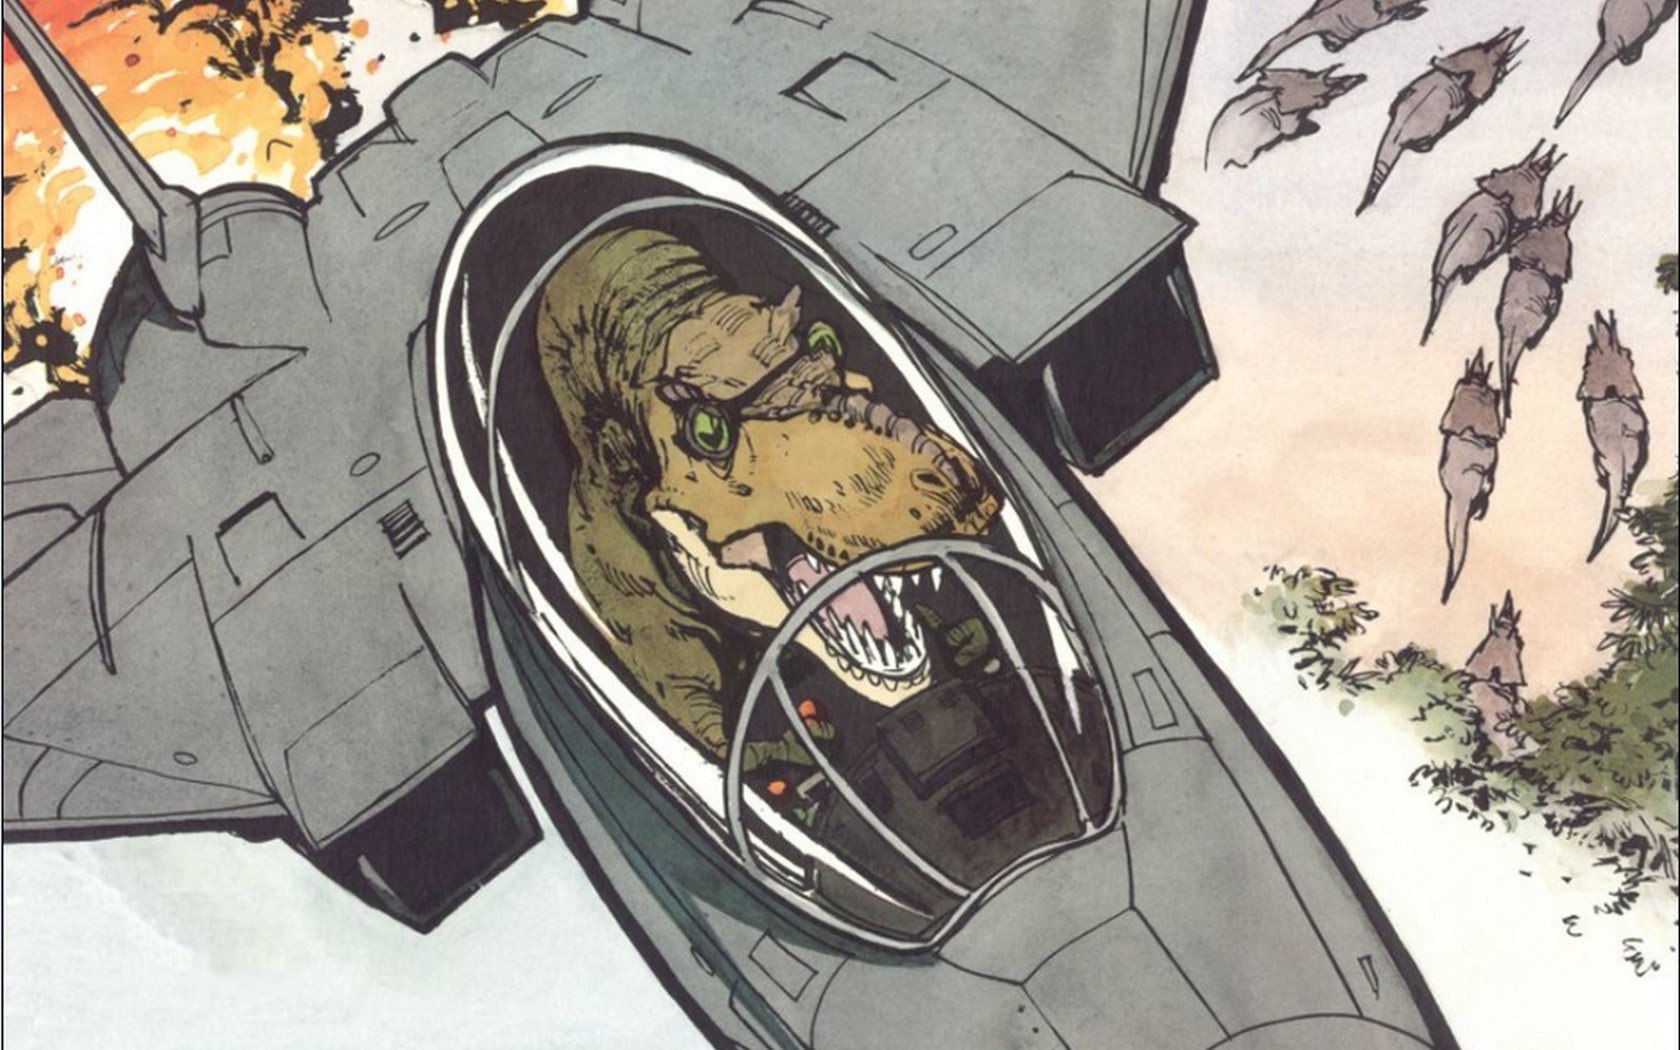
\includegraphics[width=0.80\textwidth]{placeholder}
%\caption[BDT output from the electron identification MVA.]{\temp(stuff), reproduced from\cite{eleMVA}}
%\label{fig:eleMVA}
%\end{figure}

\begin{table}[h]
\centering
\begin{tabular}{|c|c|}
\hline
\multicolumn{2}{|c|}{$5 < p_{T} < 10 GeV$} \\
$0 < |\eta_{SC}| < 0.8 $ & 0.47\\
$0.8 < |\eta_{SC}| < 1.479 $ & 0.004\\
$1.479 < |\eta_{SC}| $& 0.295\\
\hline
\multicolumn{2}{|c|}{$10 GeV < p_{T}$} \\
$0 < |\eta_{SC}| < 0.8 $& 0.5\\
$0.8 < |\eta_{SC}| < 1.479 $& 0.12\\
$1.479 < |\eta_{SC}| $& 0.60\\
\hline
\end{tabular}
\caption[The electron identification criteria.]{The electron identification
criteria. An electron passes the identification stage if the output of its MVA
is greater than the indicated value.}
\label{tab:eleCuts}
\end{table}

The momenta of the electrons is corrected using simulation by applying an
energy smearing technique in order to reproduce the calorimeter resolution
conditions observed in data. Additionally, the energy scale of the electron
superclusters in the data is corrected to match those observed in a Monte Carlo
sample by applying corrections in electrons in $(\eta, R9)$ bins. The
mismeasurement is slight, but time dependent, so the corrections are applied in
a run-range dependent manner.

Additionally, the ECAL energy measurement is corrected using a multivariate
regression technique designed original for the $H\rightarrow \gamma \gamma$
analysis~\cite{HggRegression}. The regression is based on Boosted Decision
Trees, implemented in the TMVA toolset~\cite{BDTs, BDTs2, TMVA}. Training is done using a
Drell-Yan Monte Carlo sample, splitting barrel and endcap electrons into two
separate training categories.  A wide variety of ECAL variables are used in the
process, from shower shape variables and cluster shapes to energy, momenta, and
location measurements.  The regression is designed to correct the simulated
electrons' ECAL energy back to their generated values, from either the raw
supercluster energy (in the barrel) or the supercluster plus preshower energies
(in the endcap). The net effect is an increase in the invariant mass resolution,
especially when one or both electrons are located in the
endcaps~\cite{zzHiggsMoriond}.

All electrons are required to have a fully corrected $p_T >7~GeV$ and to fall
within $|\eta|<2.5$.

\subsection{Muons}
\label{sub:muDef}
The muons utilized in this analysis are selected using a highly efficient set of
criteria, as the risk of fake muons is much lower than that of fake electrons.
As a result, only loose criteria are required to choose real muons while
eliminating a large fraction of the fakes. The muons are required to be
reconstructed via the Global or Tracker reconstruction algorithms (as described
in Chapter~\ref{chapter:eventReco}). In addition, the muons are required to be
identified as muons within the particle flow algorithm\cite{pflow}. Within this algorithm,
a tiered approach to muon identification is taken to ensure that both prompt and
secondary (from a jet) muons are identified with high efficiency. Different
criteria are placed on the muon identification based on whether or not the muon
is isolated or non-isolated. The classification is based on an isolation value
calculated by summing the transverse energy and energy from the tracks and
calorimeter deposits around the muon, within a cone of $\Delta R \le 0.3$. If the
total amount of energy within this cone is less than 10\% of the muon $p_T$, the
loosest criteria are applied to their identification. To be classified as a
PF-muon, there must exist only a valid fit between the tracks in the muon and
inner tracking systems. The muons used in this analysis are expected to be well
isolated, and should in general fall into this category. However, less isolated
prompt muons can still be identified through the so-called PF-loose or PF-tight
criteria. These rely on measurements on the number of muon chamber hits, pattern
matching between tracks and calorimeter deposits, and compatibility between
tracker and muon tracks~\cite{pflowMuons}.

Momentum scale of the muons is calibrated using the \emph{Rochester correction}
method~\cite{rochester}. In this method, corrections are applied to both data
and simulated events, so that the average value of $1/p_{T}$ matches that of a Z
decay as observed by a perfectly aligned CMS. These corrections are applied in
bins of $(Q, \eta, \phi)$, to remove the effects of poorly modeled magnetic
field or incorrect chamber alignments.

Muons are required to have a corrected $p_T >5~GeV$ and to fall within
$|\eta|<2.4$.

\subsection{Scale factors}
\label{sub:scale_factors}
Lepton reconstruction, identification, and isolation efficiencies differ
slightly between data and MC simulation, due to slight inherent differences
between real and simulated detector performance. In order to correct for these
slight differences, the lepton efficiencies are measured in both, compared, and
corrected in the MC samples. The efficiency measurements are done using the
\emph{tag and probe} method. In this method, an independent sample of
Z bosons is selected, by finding opposite sign, same flavor leptons with
invariant mass consistent with that of a  \Z boson. One lepton (called the
\emph{tag}) is required to pass a tight selection criteria, helping to ensure
the purity of the \Z sample. The other leg, called the \emph{probe} is initially
selected using only a loose criteria. This leg is then passed through the
various selection criteria (the identification, isolation, and SIP requirements
especially). After each cut is applied, the candidates are sorted into passing
and failing collections, the Z peak (and the small amount of QCD background) are
fit, and the resulting efficiencies are extracted. The process is done in both
data and Monte Carlo samples, and the ratios (as a function of $p_T$ and
$\eta$ are shown in figure~\ref{fig:tnpResults} (reproduced
from~\cite{zzAN}).  The Monte Carlo simulations are corrected in scale
by applying, for each lepton, the data/MC weight factor for the associated
($p_T, \eta$) bin.  In general, agreement between the simulations and the
observed leptons is excellent, differing only at the percent level. 

The dominant systematic uncertainties on the tag in probe method lie in how the
background and Z peak are modelled. Because the efficiency values
are extracted via a background-subtracted fit, these tails can have a
considerable effect on the final values. A conservative systematic is evaluated
by scaling the number of events in the tails up and down by a factor of two, 
recalculating the efficiency, and taking the difference from the central value
as the systematic uncertainty. Additionally, a 1\% effect is added in quadrature
to account for the shape of the \Z pole. The size of these uncertainties is
summarized in section~\ref{sec:systematics}.

\begin{figure}[h] \centering
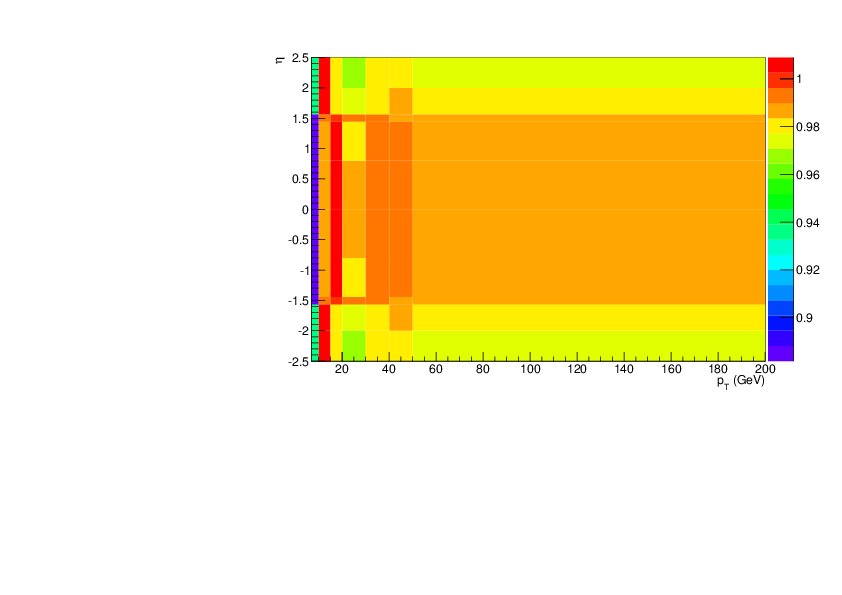
\includegraphics[width=0.60\textwidth]{ele_tnp_corrections} 
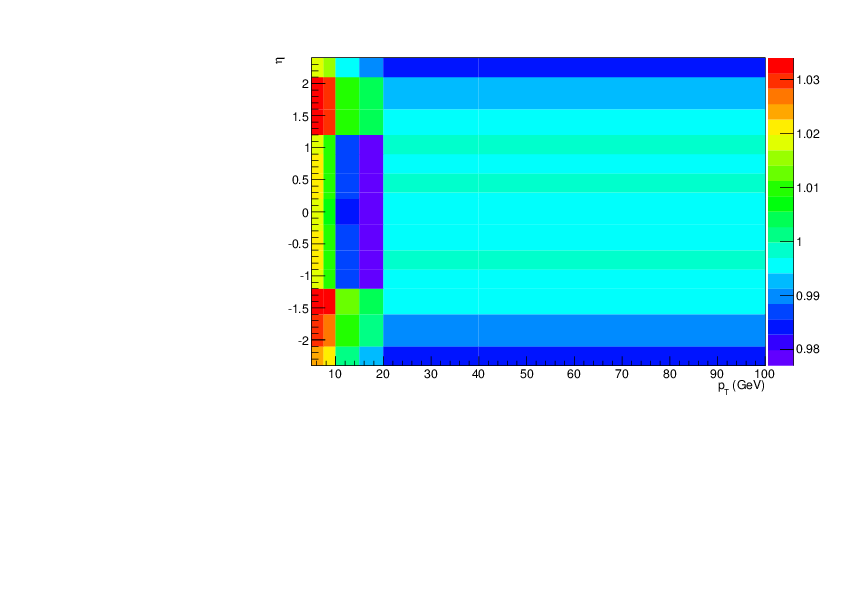
\includegraphics[width=0.60\textwidth]{mu_tnp_corrections}\\
\caption[Ratio of lepton efficiencies between data and monte carlo simulations
for electrons and muons.]{Ratio of lepton efficiencies between data and Monte Carlo simulations
    for electrons (top) and muons (bottom). Results are reproduced
from~\cite{zzAN}.}
\label{fig:tnpResults}
\end{figure}

\section{Pile-up Reweighing}
\label{sub:pileup}
Because the simulated samples were produced with a pile-up scenario
(which does not match the overall scenario in the final data samples), the
simulated samples must be reweighted. By giving the simulated events a slightly
higher or lower weight factor in the final distributions, it is possible to
create a simulated sample whose net pile-up closely resembles that which is
observed in the data.

The distributions of the reconstructed vertices, while a good indicator of pile
up activity, are susceptible to biases coming from the trigger and vertex
finding algorithms. As a result, the ``true'' number of pile-up interactions are
used. In the Monte Carlo simulation, this number is immediately accessible. In
the data, it comes from instantaneous luminosity measurements, stored in
per-bunch-crossing per-luminosity section intervals. This measurement, combined
with the total pp cross-section, is used to determine the pile-up distribution,
as observed by CMS, as it evolves in time. The ratio between the observed and
simulated pile-up distributions for each bin in the simulated distribution tells
how those events must be weighted in order to match the observed.

To test the effectiveness of using the ``true'' pileup variables described, one
can easily check the effect on the reconstructed vertex distribution.  The
results can be seen in figure~\ref{fig:puCorrs}. After corrections, the MC
sample successfully reproduces the pile-up scenario observed in data.
\begin{figure}[h]
\centering
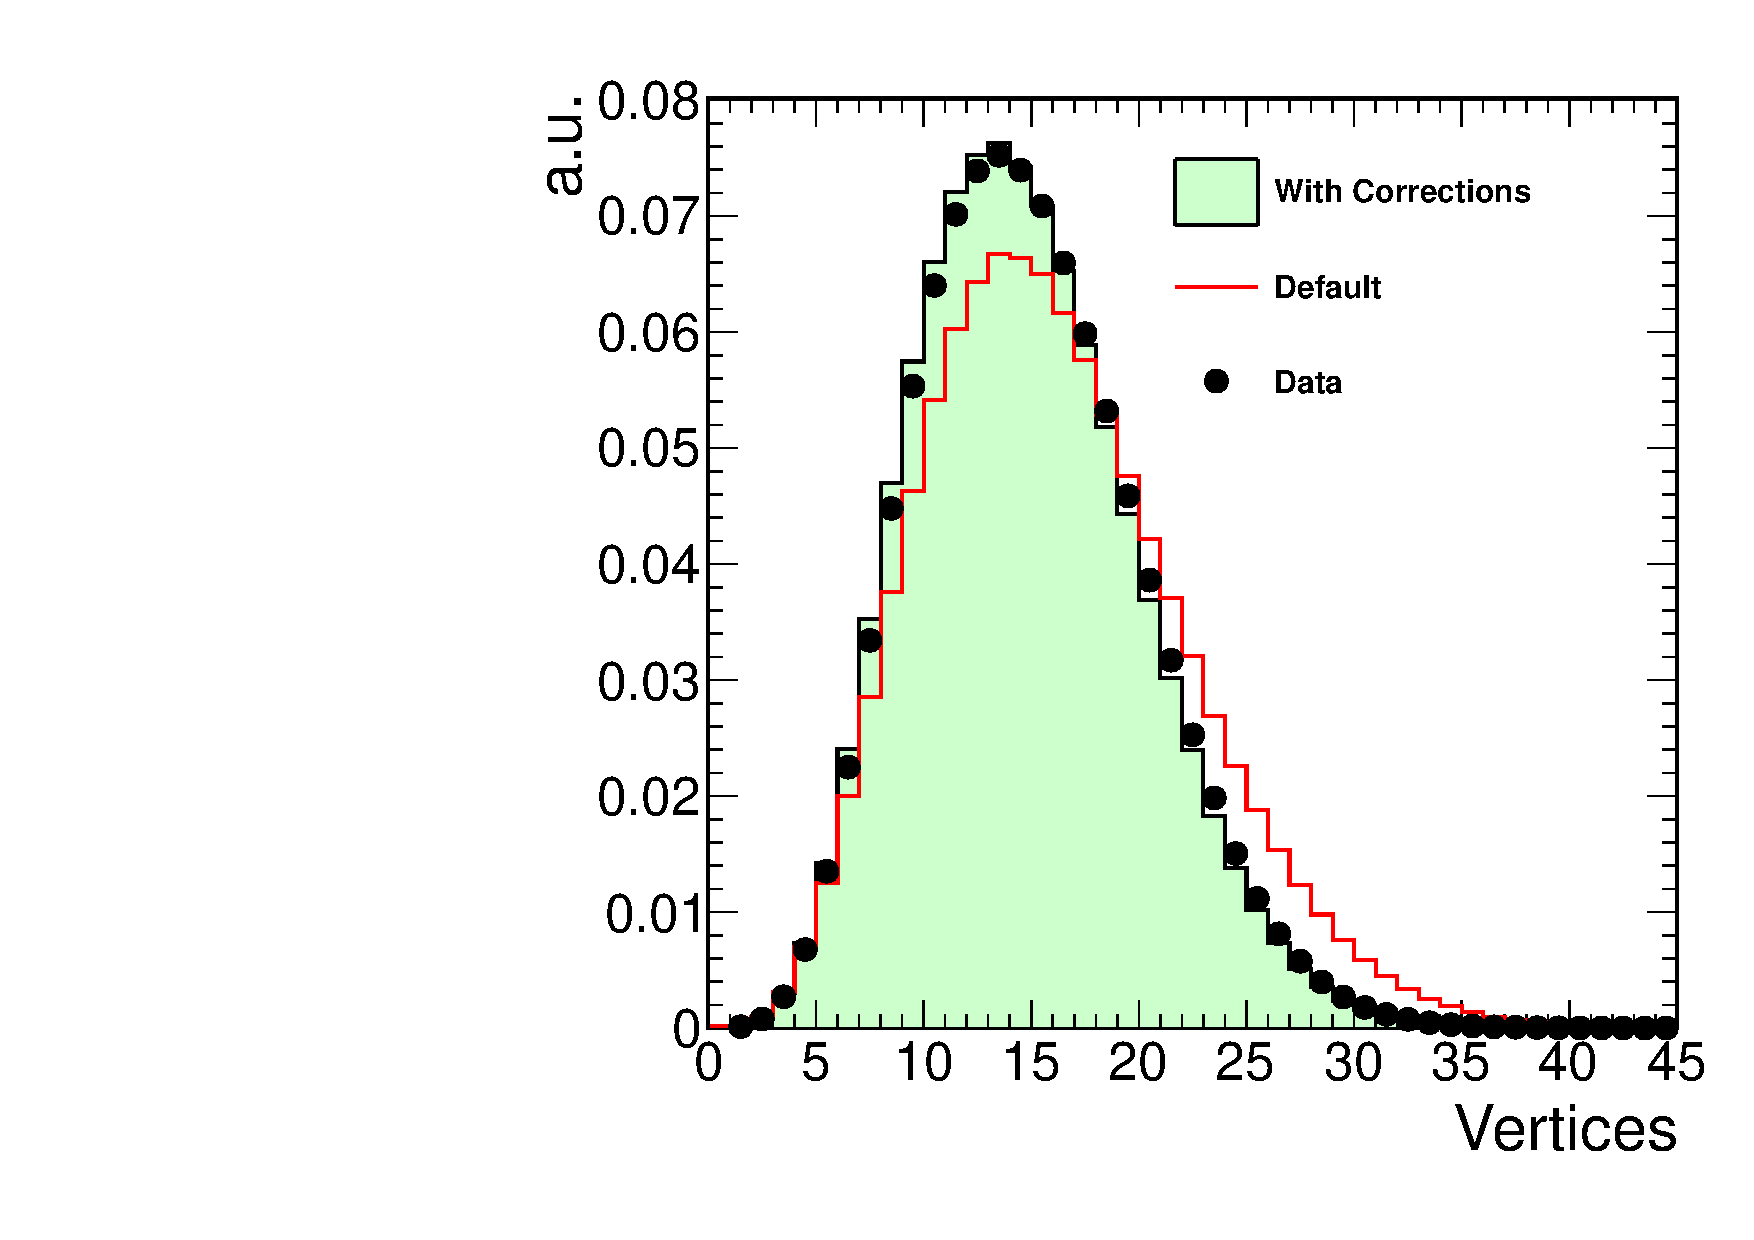
\includegraphics[width=0.80\textwidth]{pu_corrected}
\caption[The effects of pile-up corrections on the rectonstructed vertex
distribtion.]{The effects of pile-up corrections, as described in the text, on
the reconstructed vertex distribution. There is a significant improvement in the
MC-data agreement when the corrections are applied.}
\label{fig:puCorrs}
\end{figure}


\section{Background Estimation}
\label{sec:bgEst}
To estimate the reducible background contribution (coming primarily from a
Z+jets signature with a much smaller contribution from the W/Z+jet production),
a data-driven ``fake-rate method'' is utilized. In this approach, the
probability for a loosely identified lepton (interpreted physically as a jet) to
pass the full lepton selection is calculated. This fake rate is then applied to
the population of a number of subregions which are dominated by these background
physics events. This gives an estimate of the number of these events which are
expected to pass the final selection criteria.

The first step is measuring the leptonic fake rates. This is done using in a
``$\Z + 1 \ell$'' region, where one \Z boson is fully selected and there is exactly
one additional loose lepton found in the event. These leptons have the
requirements from Table~\ref{tab:looseLeps} applied, with an additional
event-level requirement of less than 20~GeV of missing transverse energy (in
order to cut down contamination from WZ production).

\begin{table}[h]
\centering
\begin{tabular}{|c|c|}
\hline
Electrons & $p_{T}>7$~GeV\\
& $|\eta|<2.5$\\
& $<2$ missing inner tracker hits\\
& $|d_{XY}| < 0.5 $~cm  \\
& $|d_{Z}| < 1.0 $~cm \\
\hline
\hline
Muons & $p_{T}>5$~GeV\\
& $|\eta|<2.4$\\
& Global OR Tracker (with $\ge$ 1 segment matched)\\
& $|d_{XY}| < 0.5$~cm  \\
& $|d_{Z}| < 1.0$~cm  \\
\hline
\end{tabular}
\caption[Loose lepton definitions.]{The criteria placed on the loose lepton objects.}
\label{tab:looseLeps}
\end{table}
The leptonic fake rates are then measured as the number of loose leptons which
pass final lepton selection (as defined in sections~\ref{sub:eleDef}
and~\ref{sub:muDef}).
\begin{equation}
    \label{eqn:fr}
    f = \frac{\textrm{Passing full selection}}{\textrm{Passing loose
    criteria}}
\end{equation}

These fake rates, as a function of lepton $p_{T}$, are depicted in
figure~\ref{fig:fakerates}. The dependence on $p_{T}$ is slight, and the fake
rates are applied in a $p_{T}$ independent manner.
\begin{figure}[h]
\centering
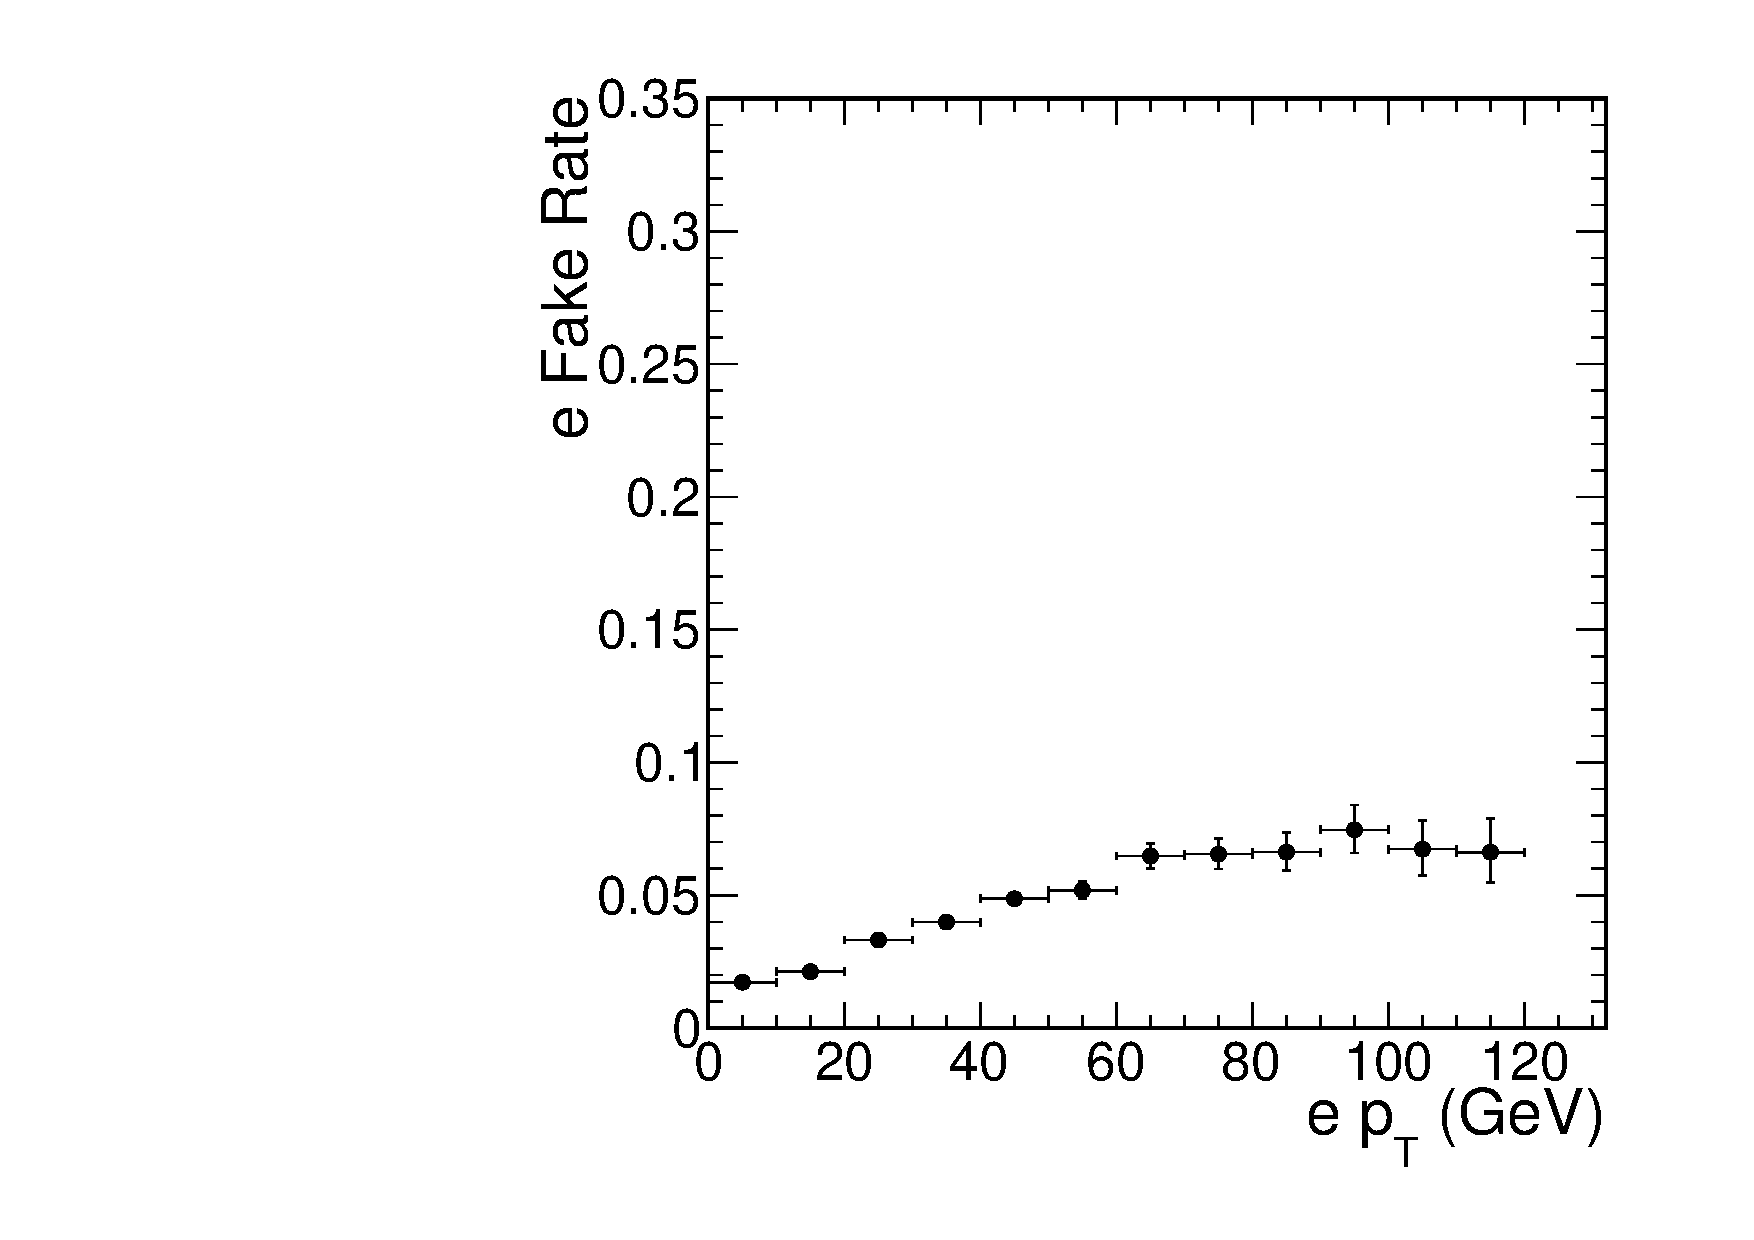
\includegraphics[width=0.45\textwidth]{ele_FR}
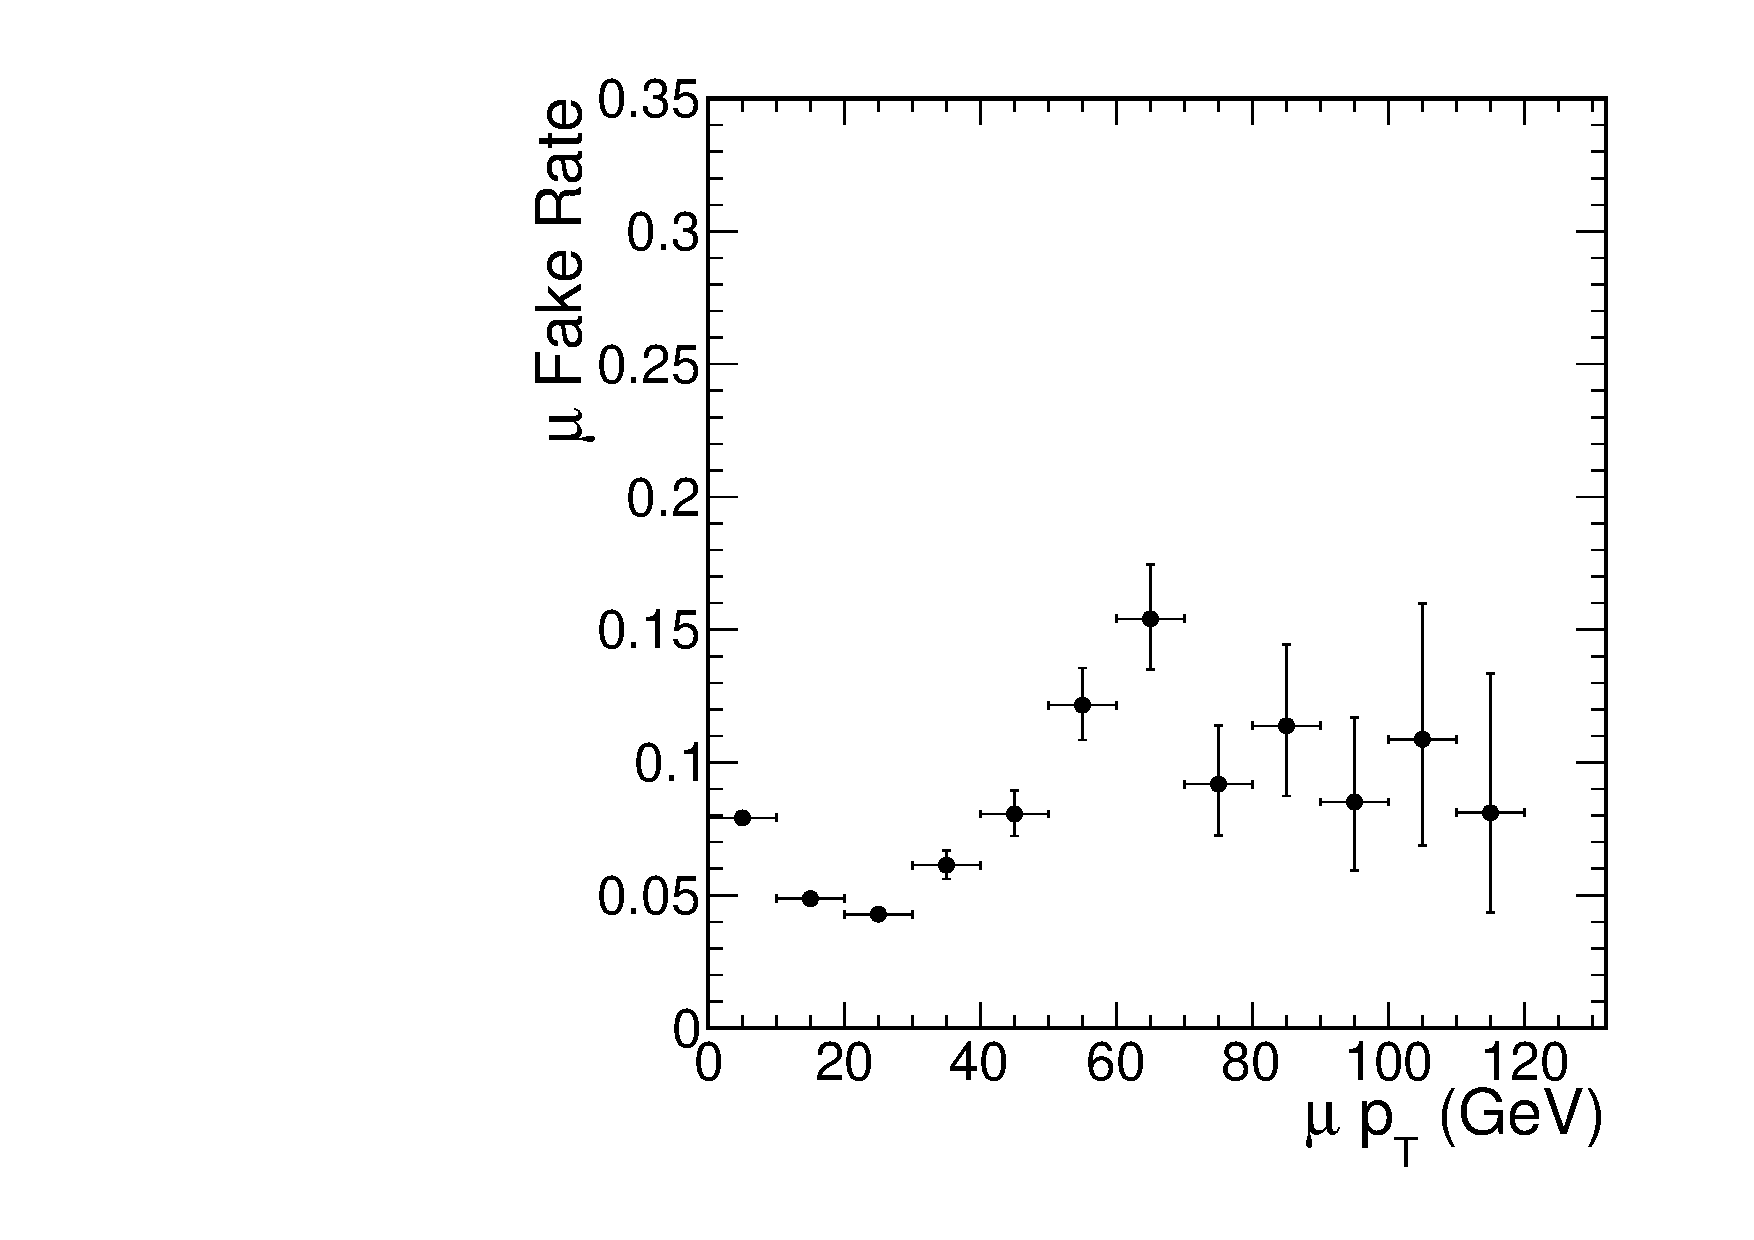
\includegraphics[width=0.45\textwidth]{mu_FR}
\caption[Leptonic fake rates used for the background estimation.]{The leptonic
fake rates, as a function of $p_{T}$ for the electrons (left) and muons (right).}
\label{fig:fakerates}
\end{figure}

In order to estimate the total background contributions due to fakes, potential
backgrounds are split into two separate regions. The first region is
composed of events which contain a fully selected Z, one lepton passing full
selection, and one loose lepton which fails the final selection criteria
(\emph{Z+1P1F}).  These regions are dominated by \Z boson production in
association with two jets, where one of the jets `fakes' a prompt lepton. In
addition, there is a small contribution of W/Z+1 jet production in this region
(though the smaller cross section restricts its impact). The second region is
composed of events with a fully reconstructed \Z boson plus two additional loose
leptons, both of which fail the final selection criteria (\emph{Z+2F}). This region is
composed almost entirely of \Z boson production. There is a negligible contamination
of ZZ in each of these regions. The population for these regions for each of the
final states (plus the combination) is shown in figures~\ref{fig:AAregions}
and~\ref{fig:AIregions}. The statistics in the simulated Drell-Yan sample has
limited statistics when an on-shell Z is required (as seen in
figures~\ref{fig:AAregions_highmass} and~\ref{fig:AIregions_highmass}). However,
the overall successful modelling of these control regions with the looser mass
requirements (Figures~\ref{fig:AAregions} and \ref{fig:AIregions}) gives confidence
in the method, as the expected physics processes are the same regardless of the
mass requirement.

\begin{figure}[h]
\centering
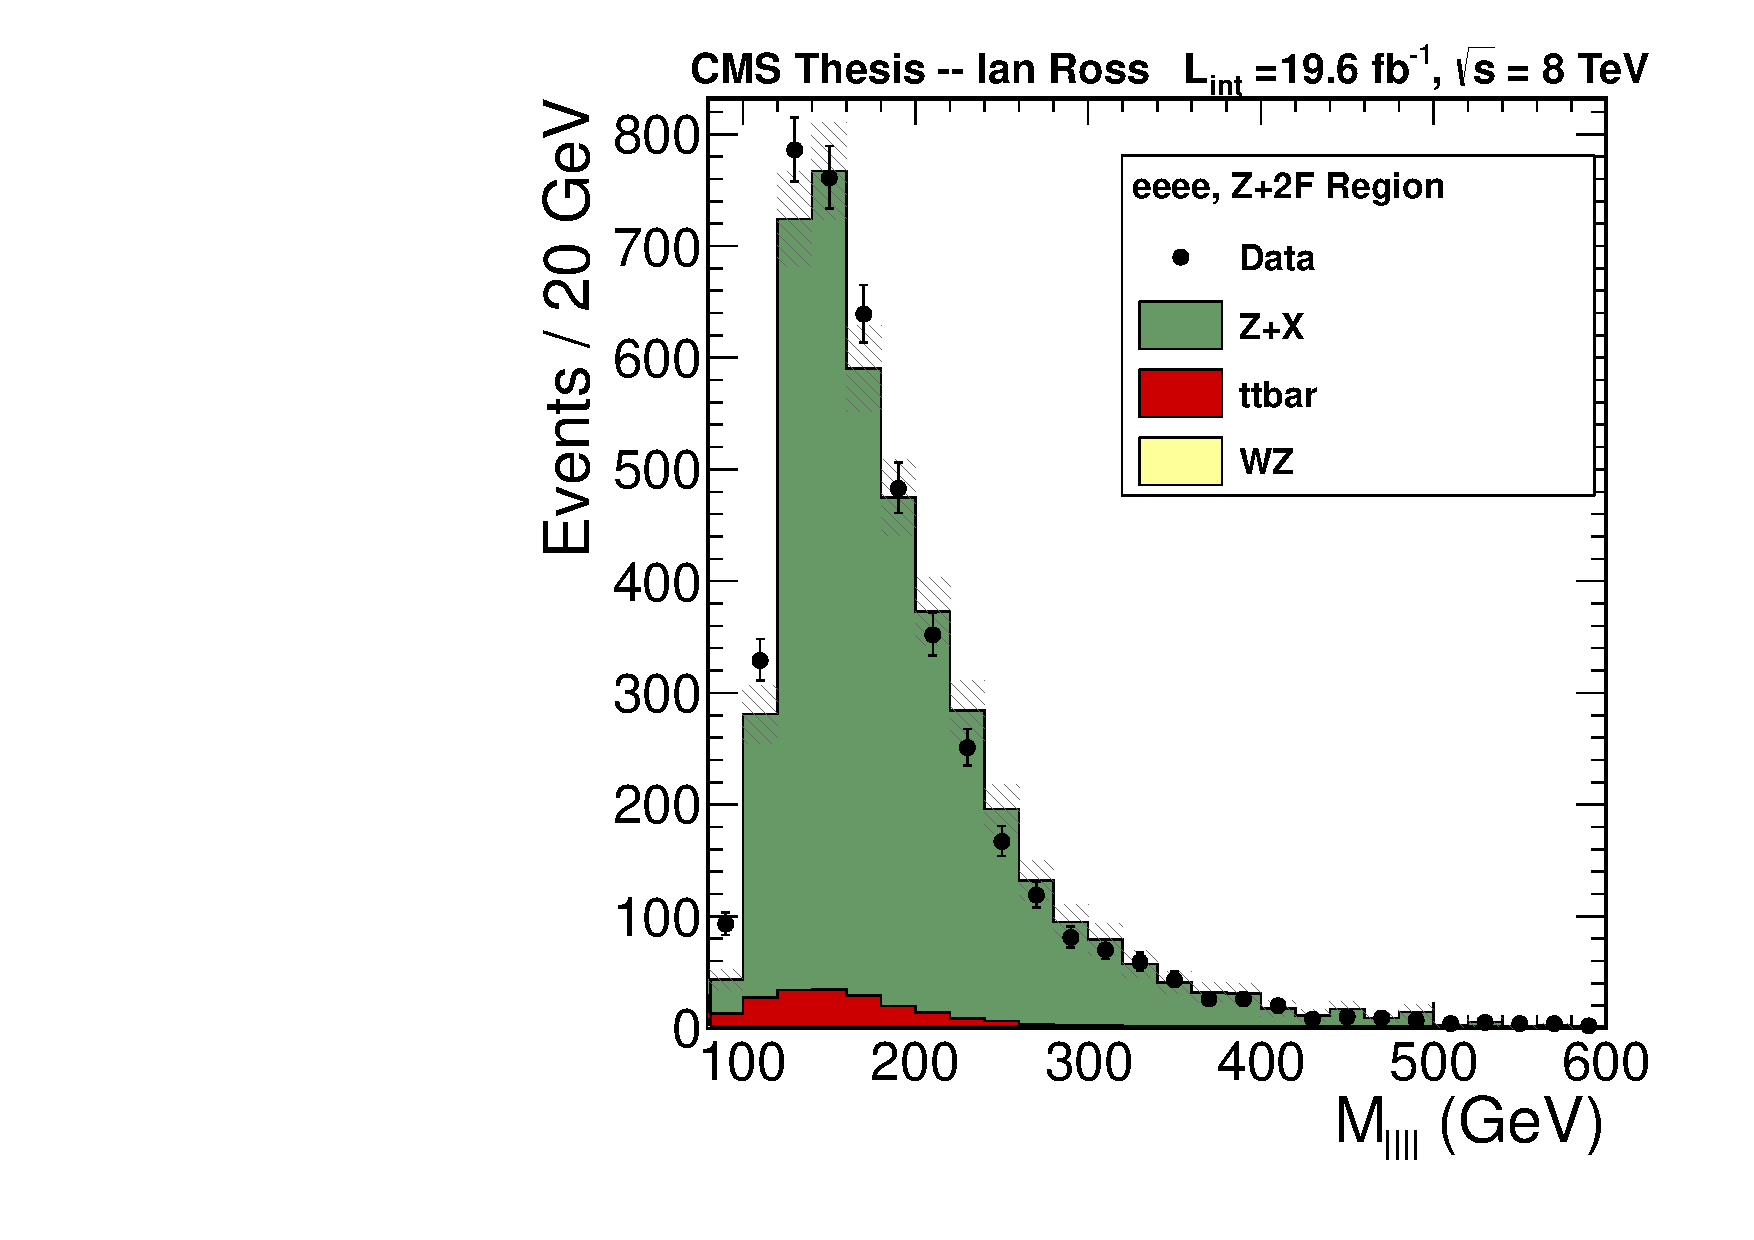
\includegraphics[width=0.45\textwidth]{eeee_AA}
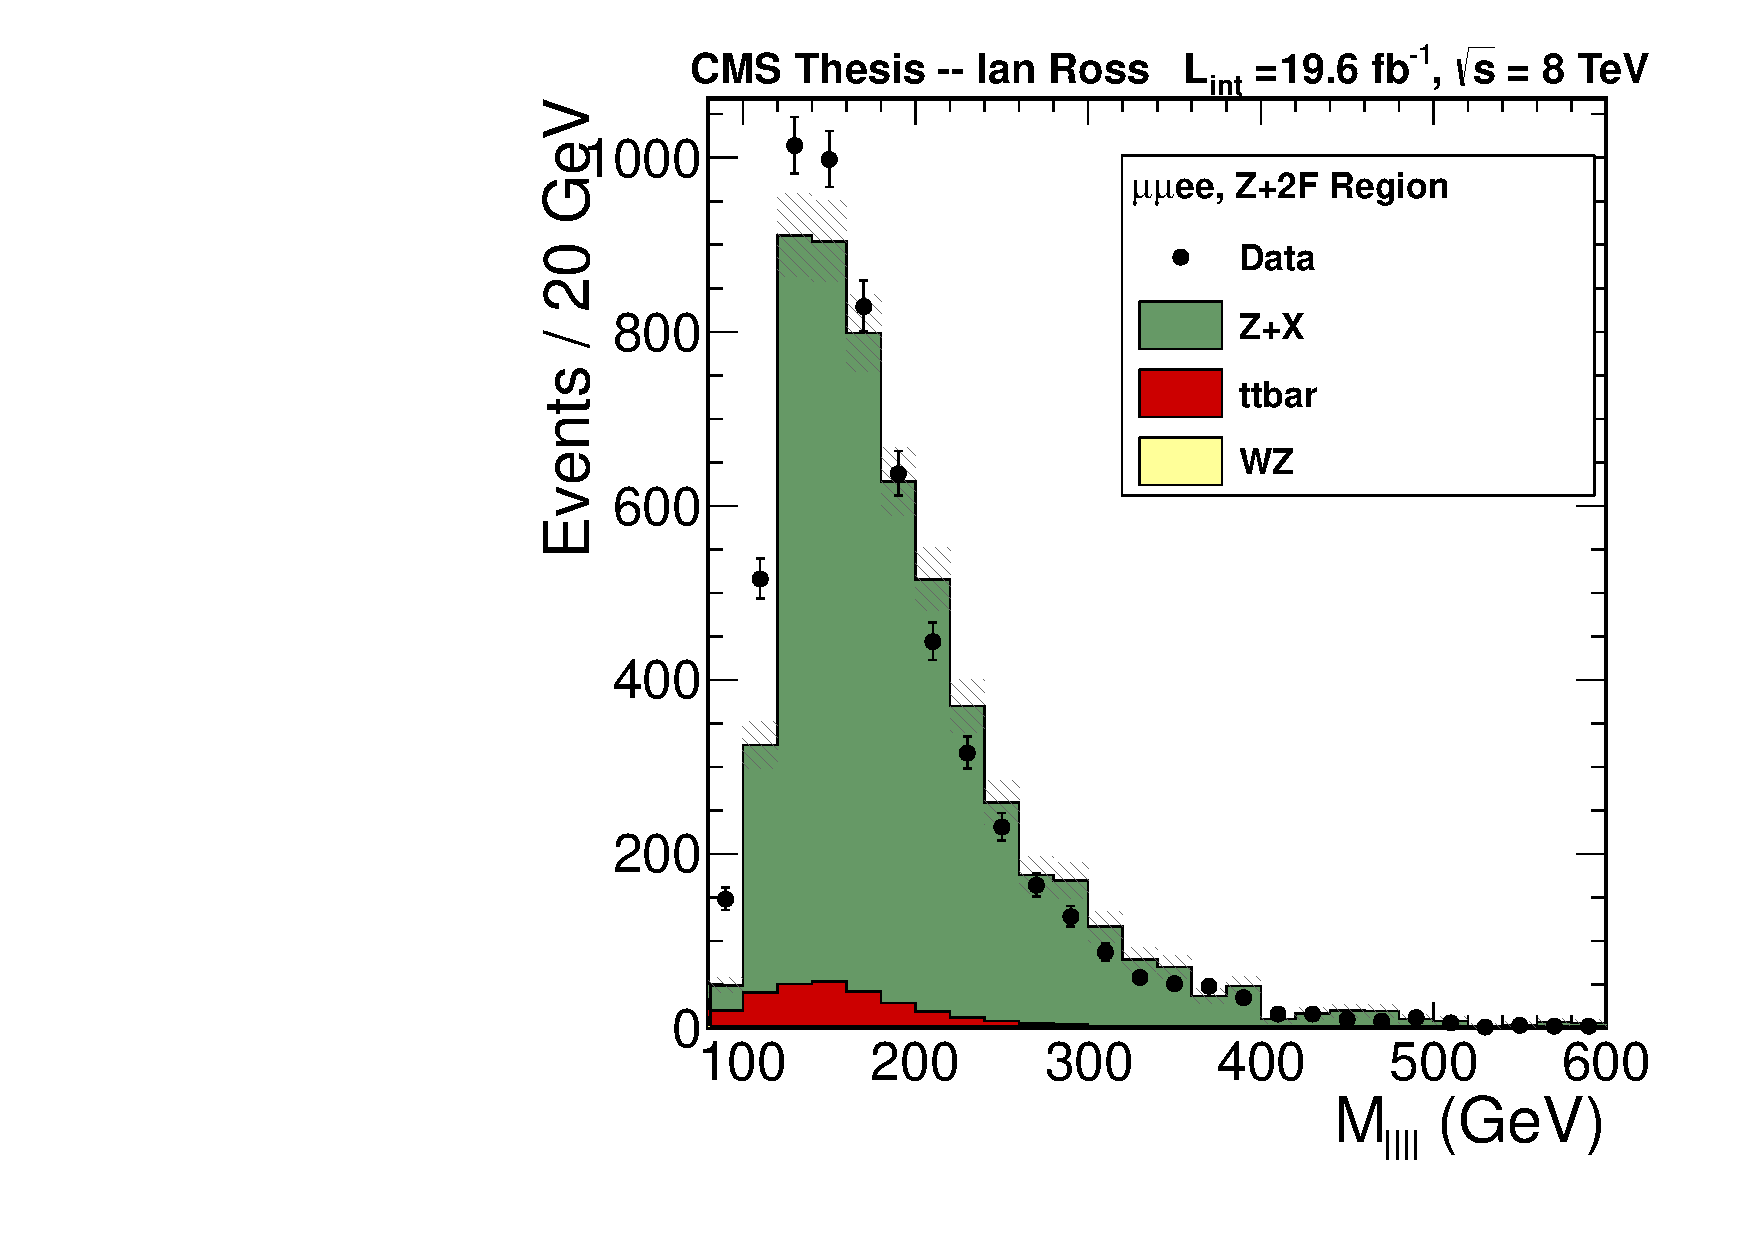
\includegraphics[width=0.45\textwidth]{mmee_AA}\\
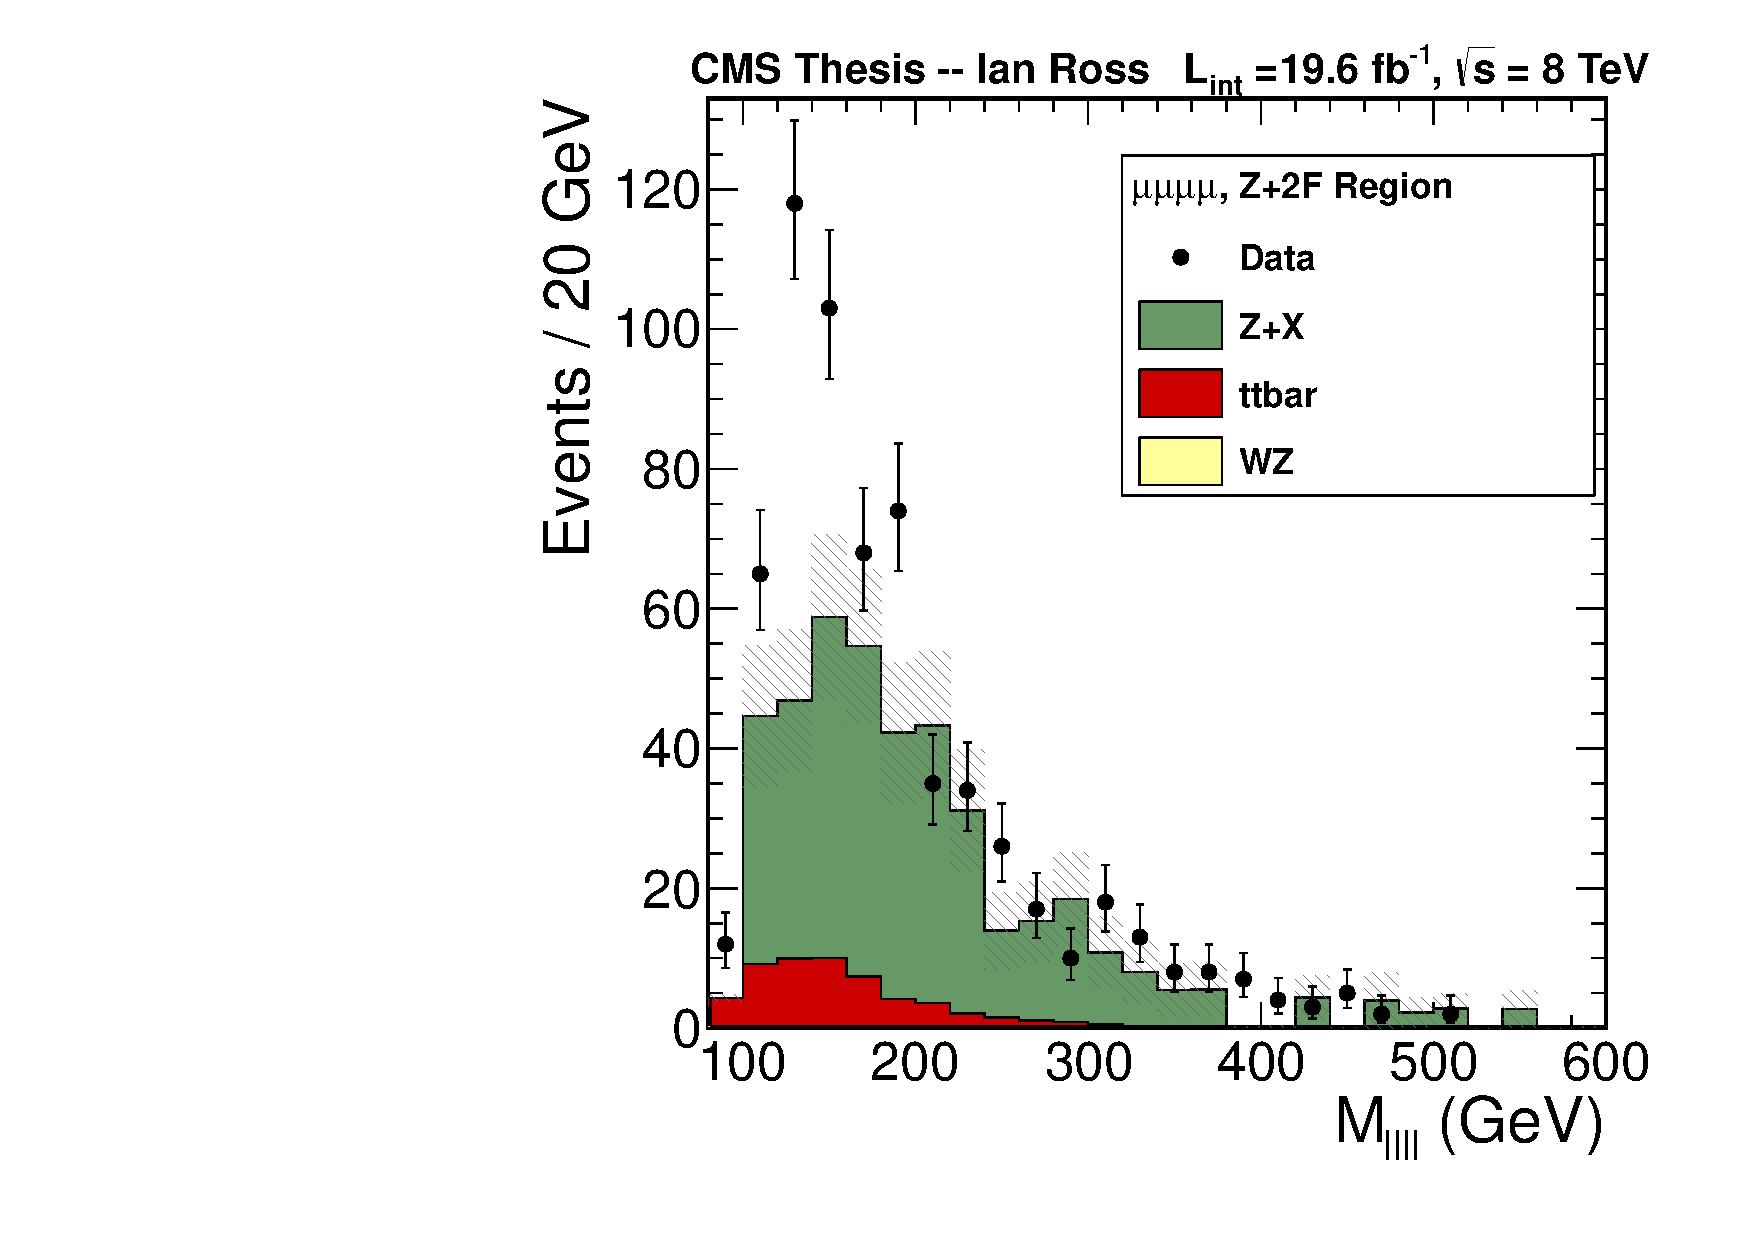
\includegraphics[width=0.45\textwidth]{mmmm_AA}
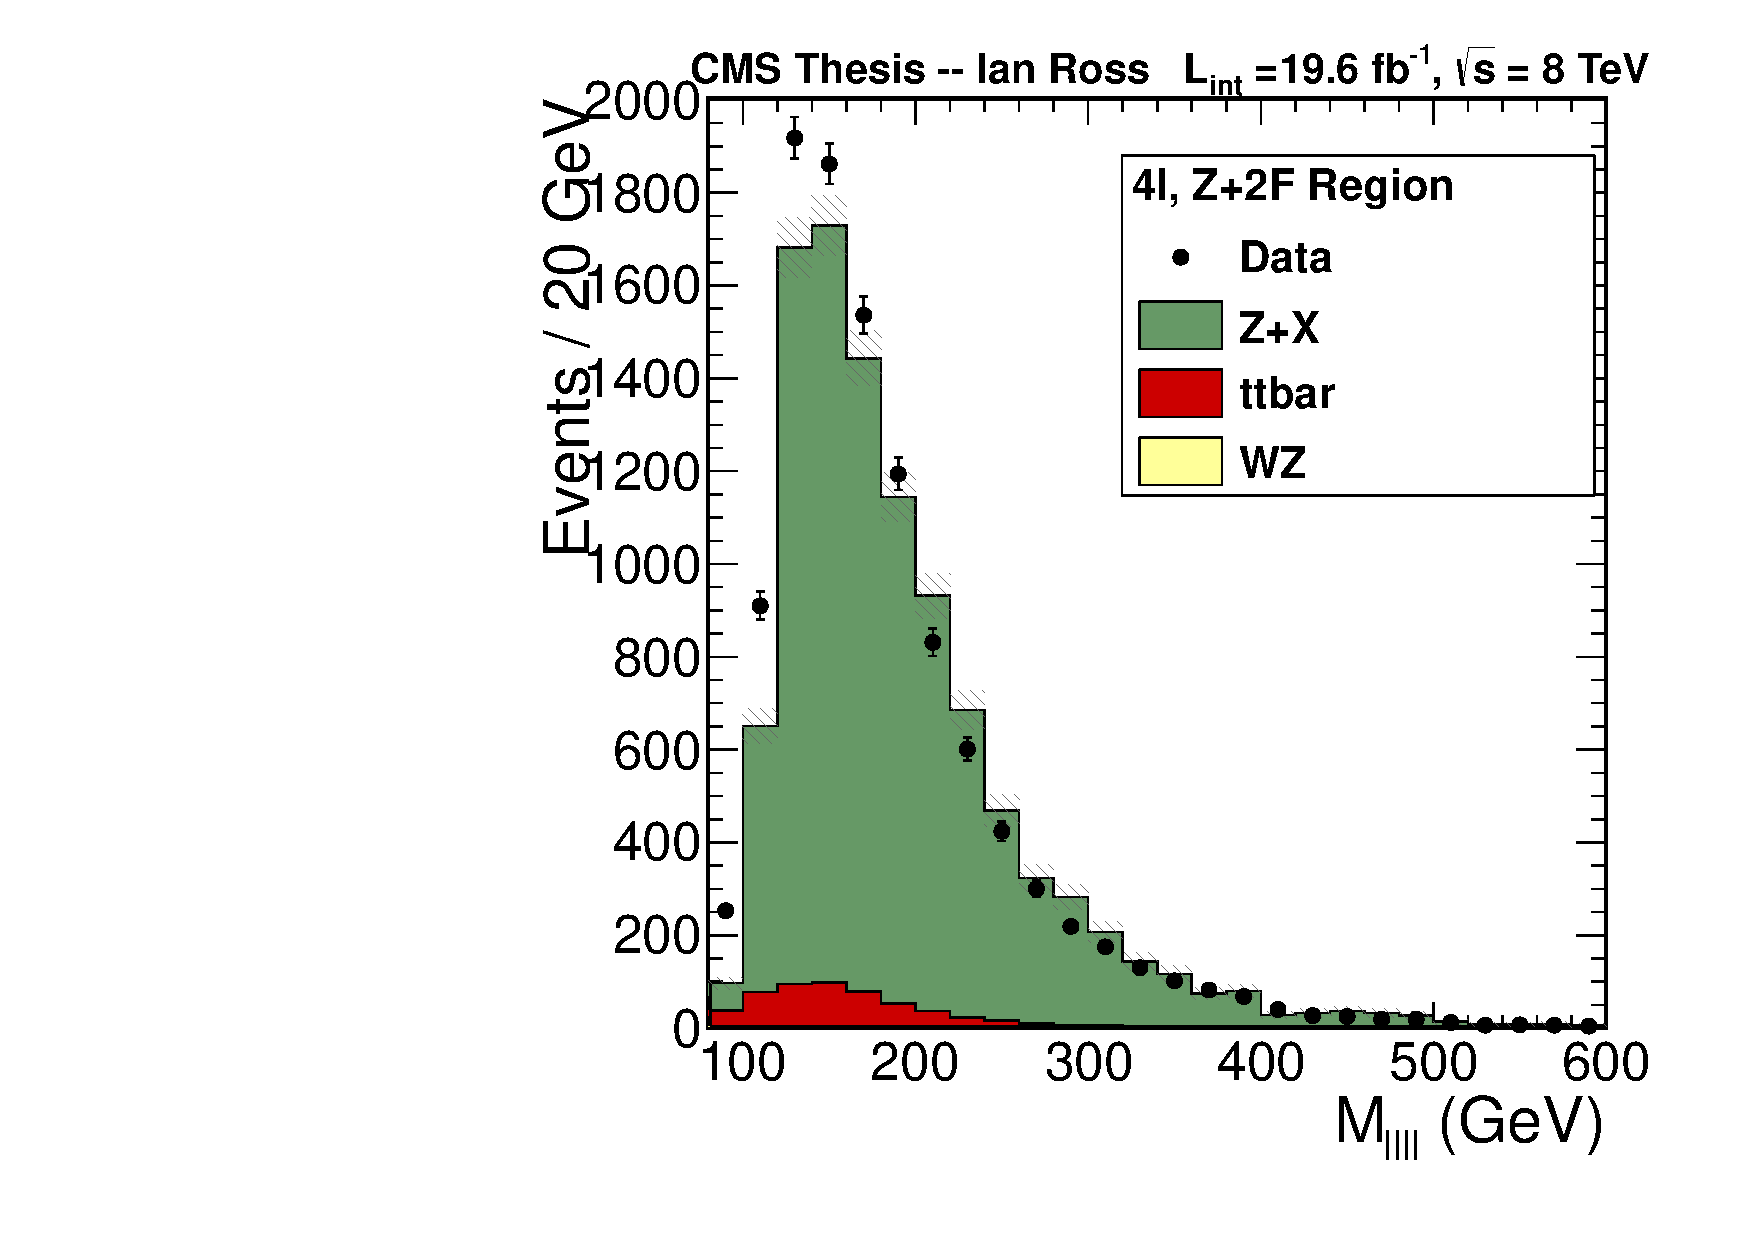
\includegraphics[width=0.45\textwidth]{4l_AA}\\
\caption[Background estimation region consisting of a \Z plus two failed
leptons.]{Background estimation region consisting of a \Z plus two failed
leptons. Counter clockwise from top right is the eeee, $\mu\mu ee$,
$\mu\mu\mu\mu$, and summed final states.}
\label{fig:AAregions}
\end{figure}

\begin{figure}[h]
\centering
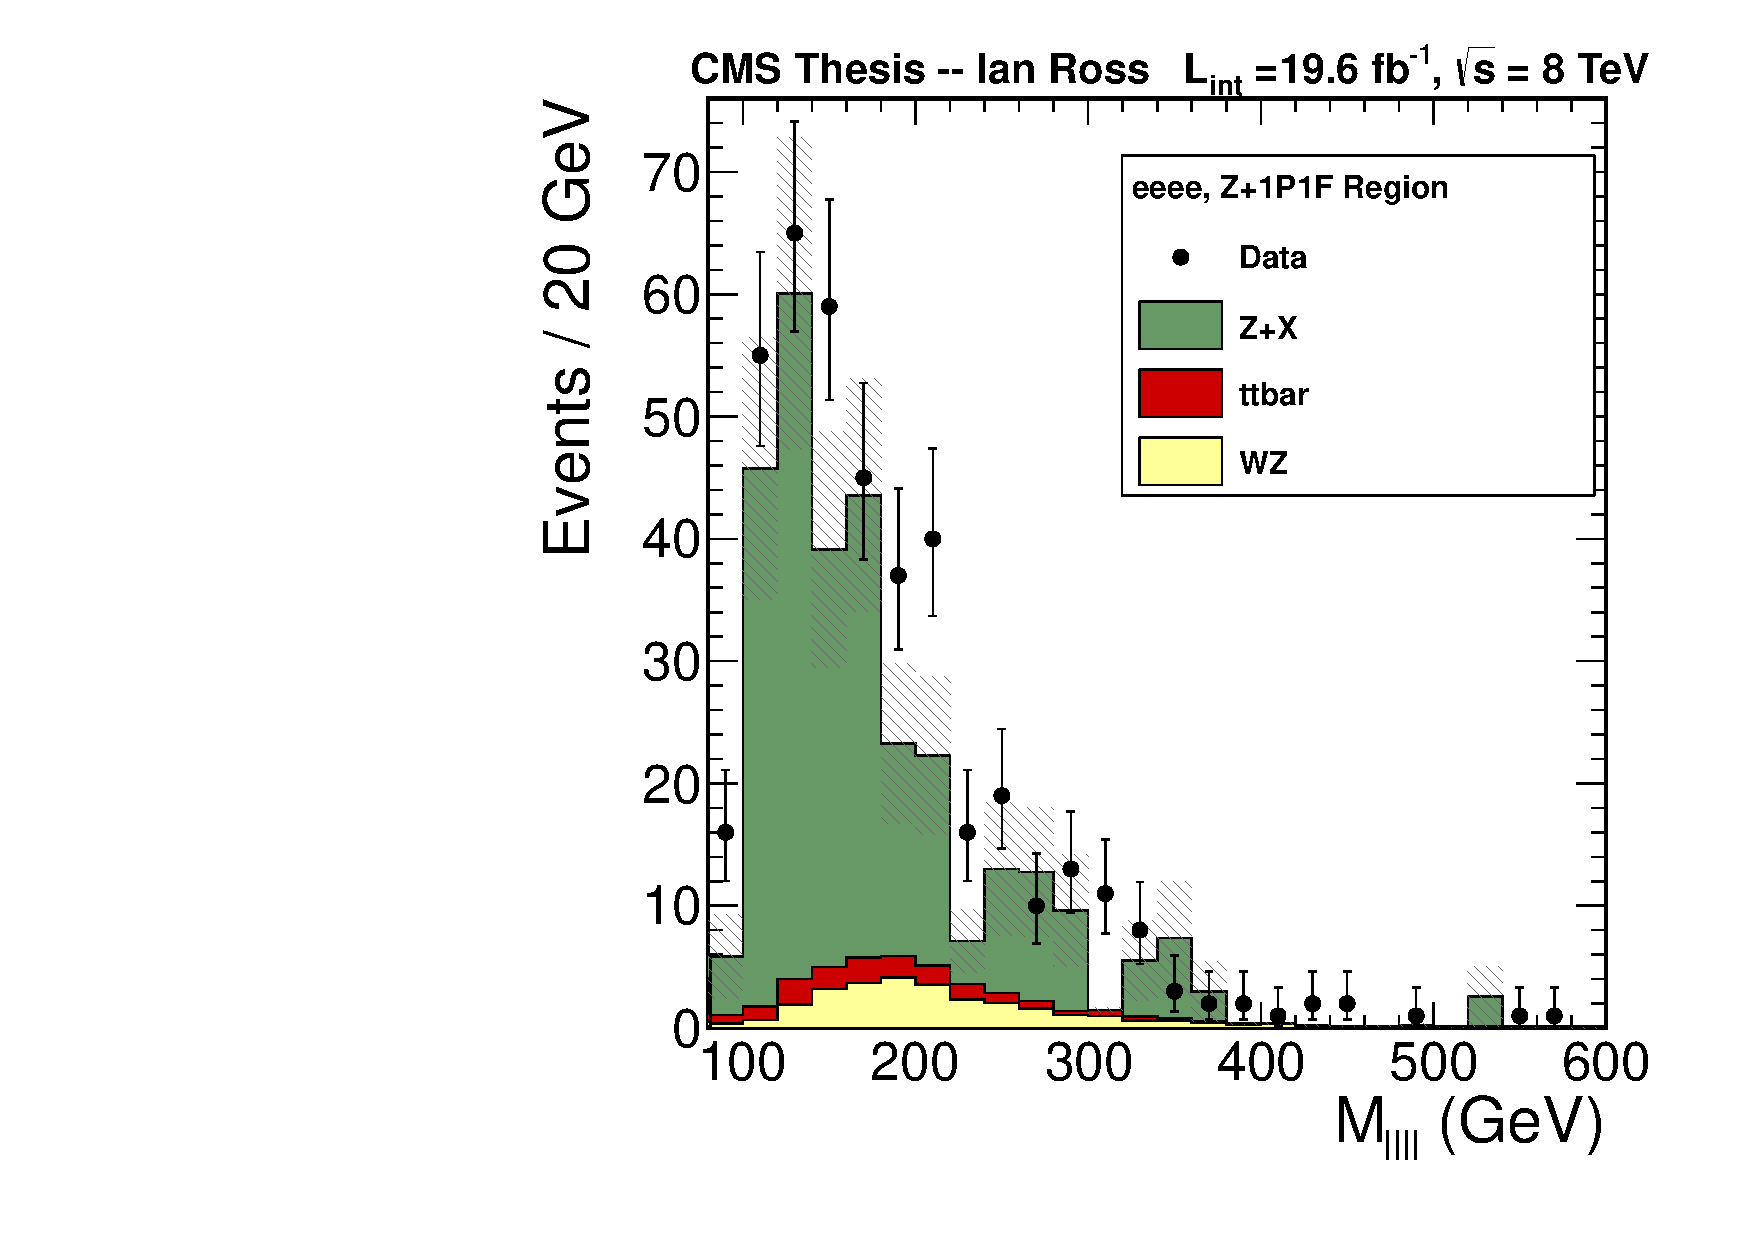
\includegraphics[width=0.45\textwidth]{eeee_IA}
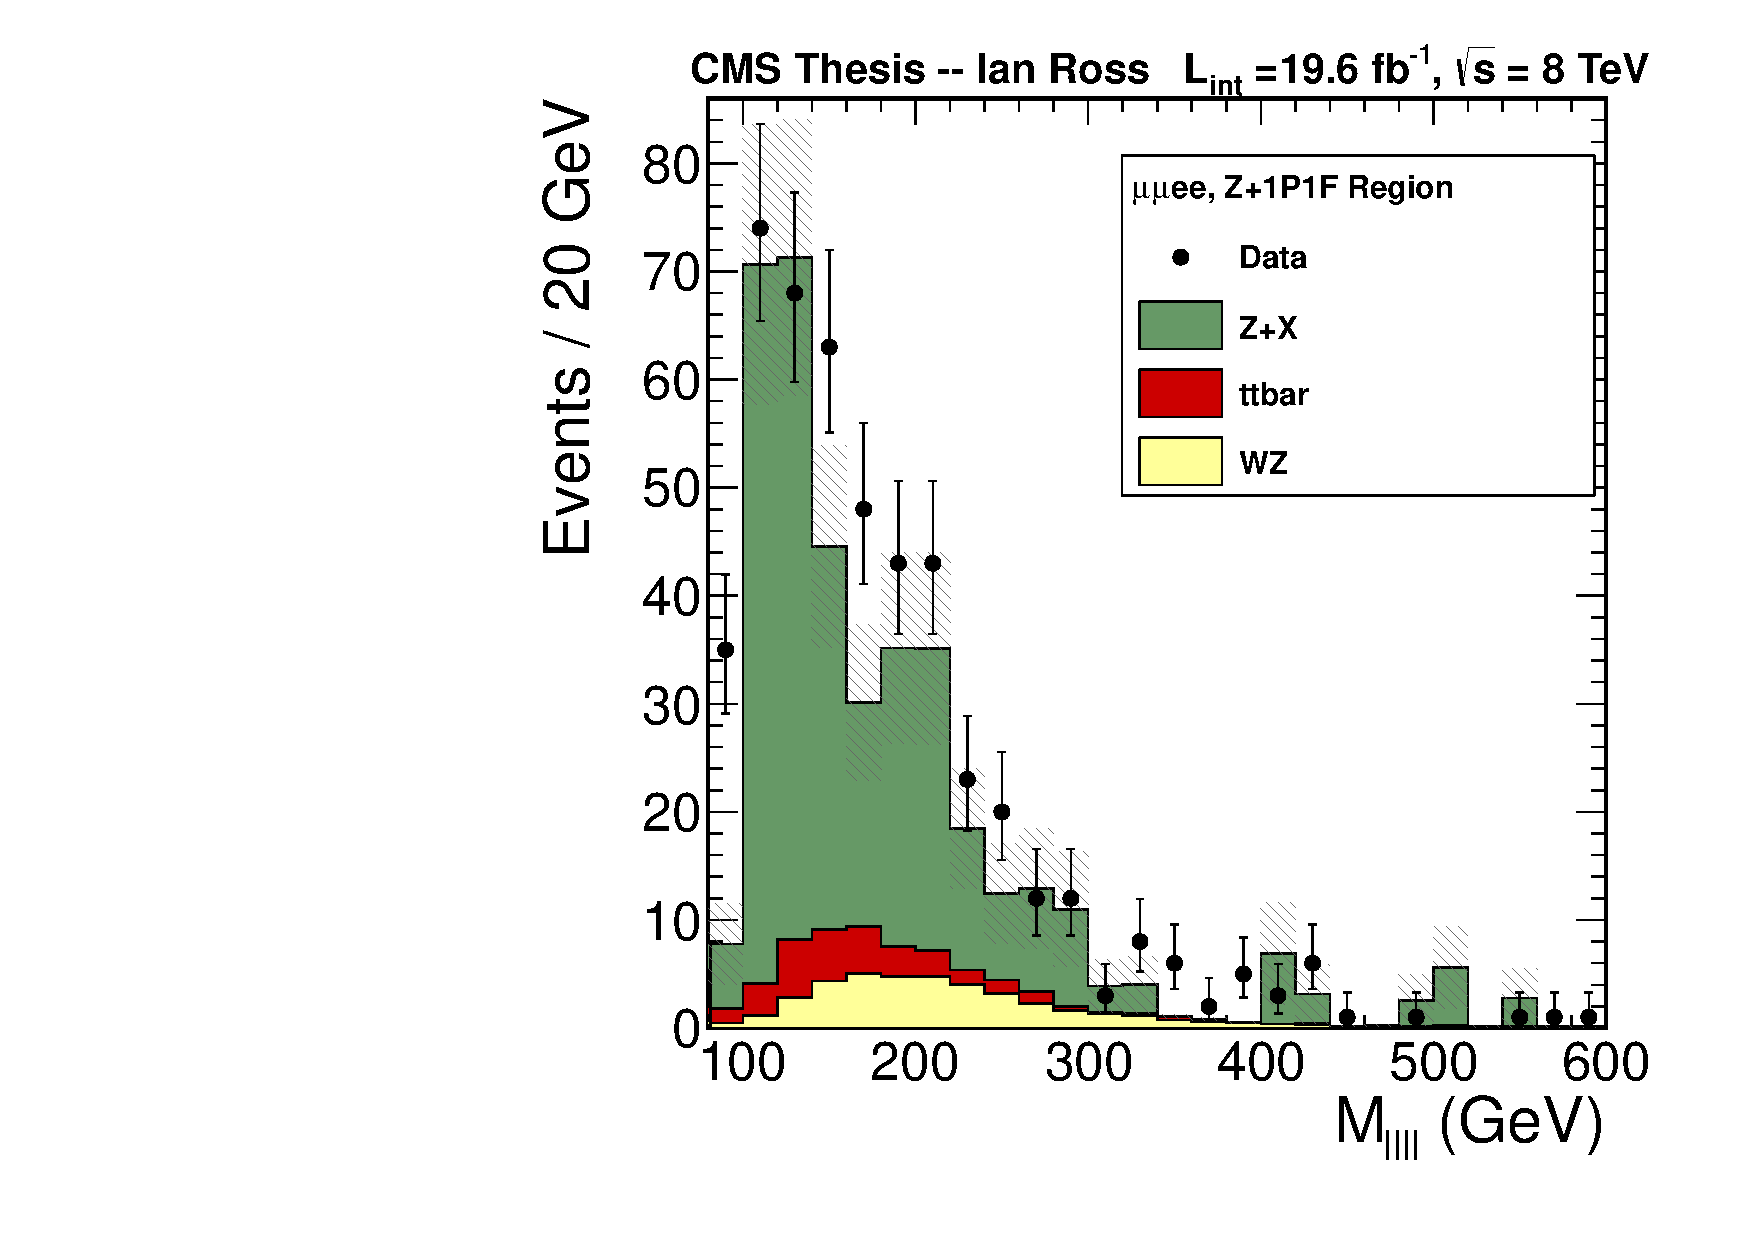
\includegraphics[width=0.45\textwidth]{mmee_IA}\\
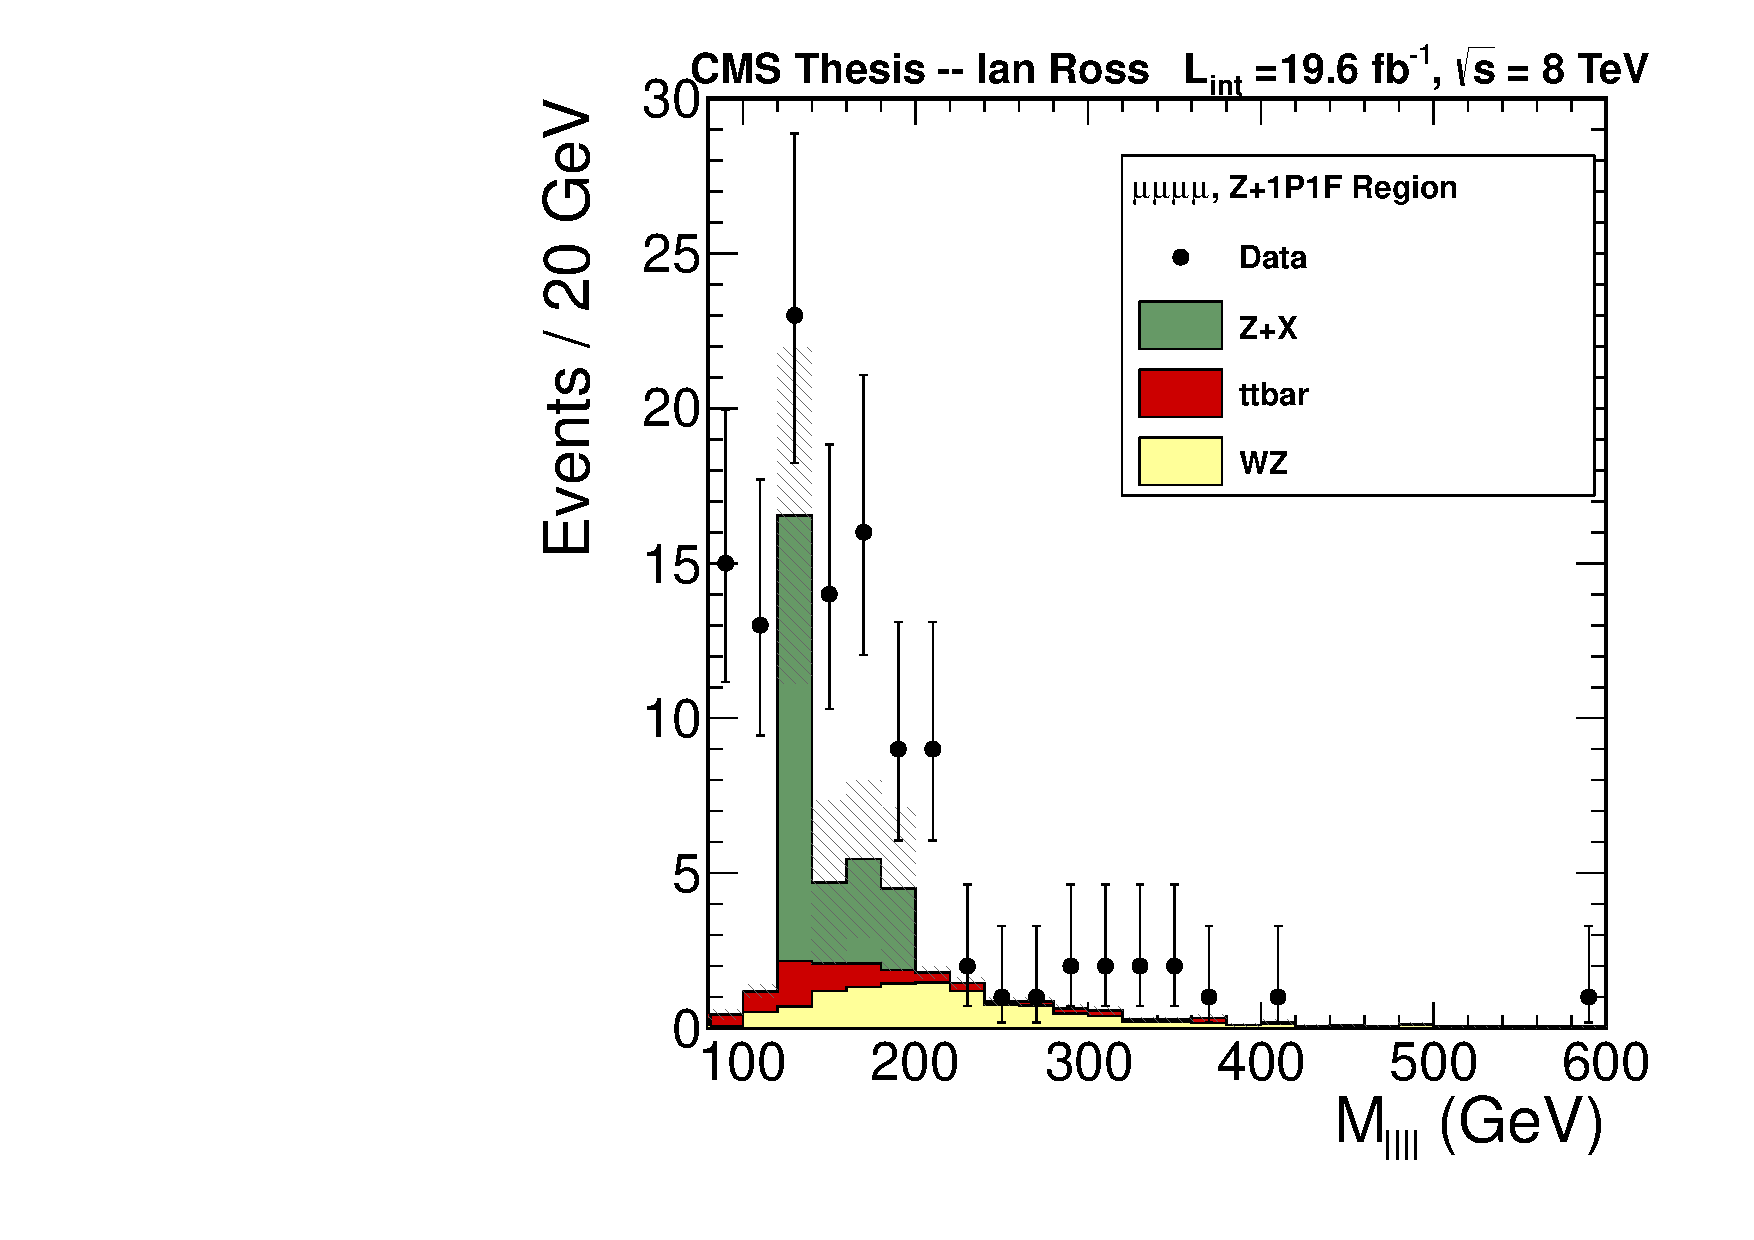
\includegraphics[width=0.45\textwidth]{mmmm_IA}
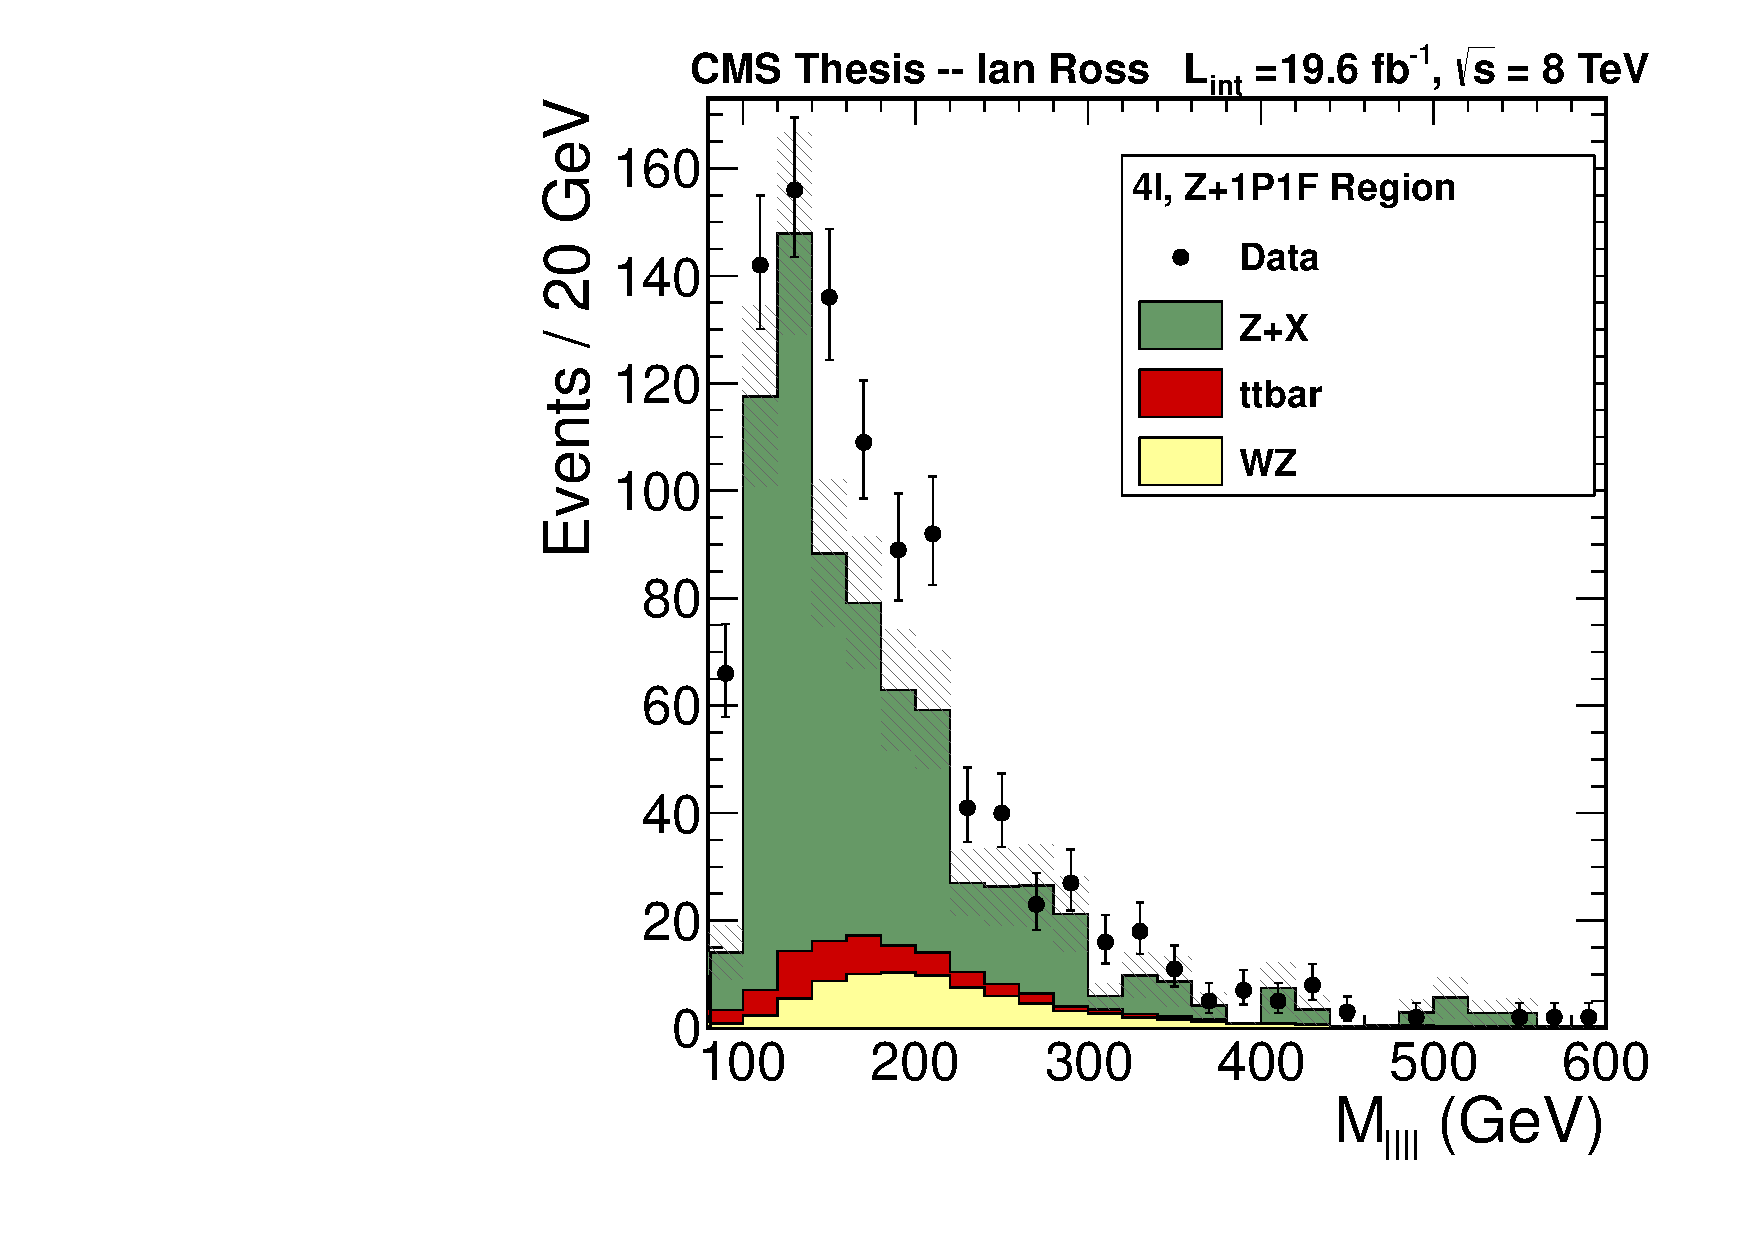
\includegraphics[width=0.45\textwidth]{4l_IA}\\
\caption[Background estimation region consisting of a \Z plus one passed and one failed
leptons.]{Background estimation region consisting of a \Z plus one passed and
    one failed leptons. Counter clockwise from top right is the eeee, $\mu\mu
    ee$, $\mu\mu\mu\mu$, and summed final states.}
\label{fig:AIregions}
\end{figure}

\begin{figure}[h]
\centering
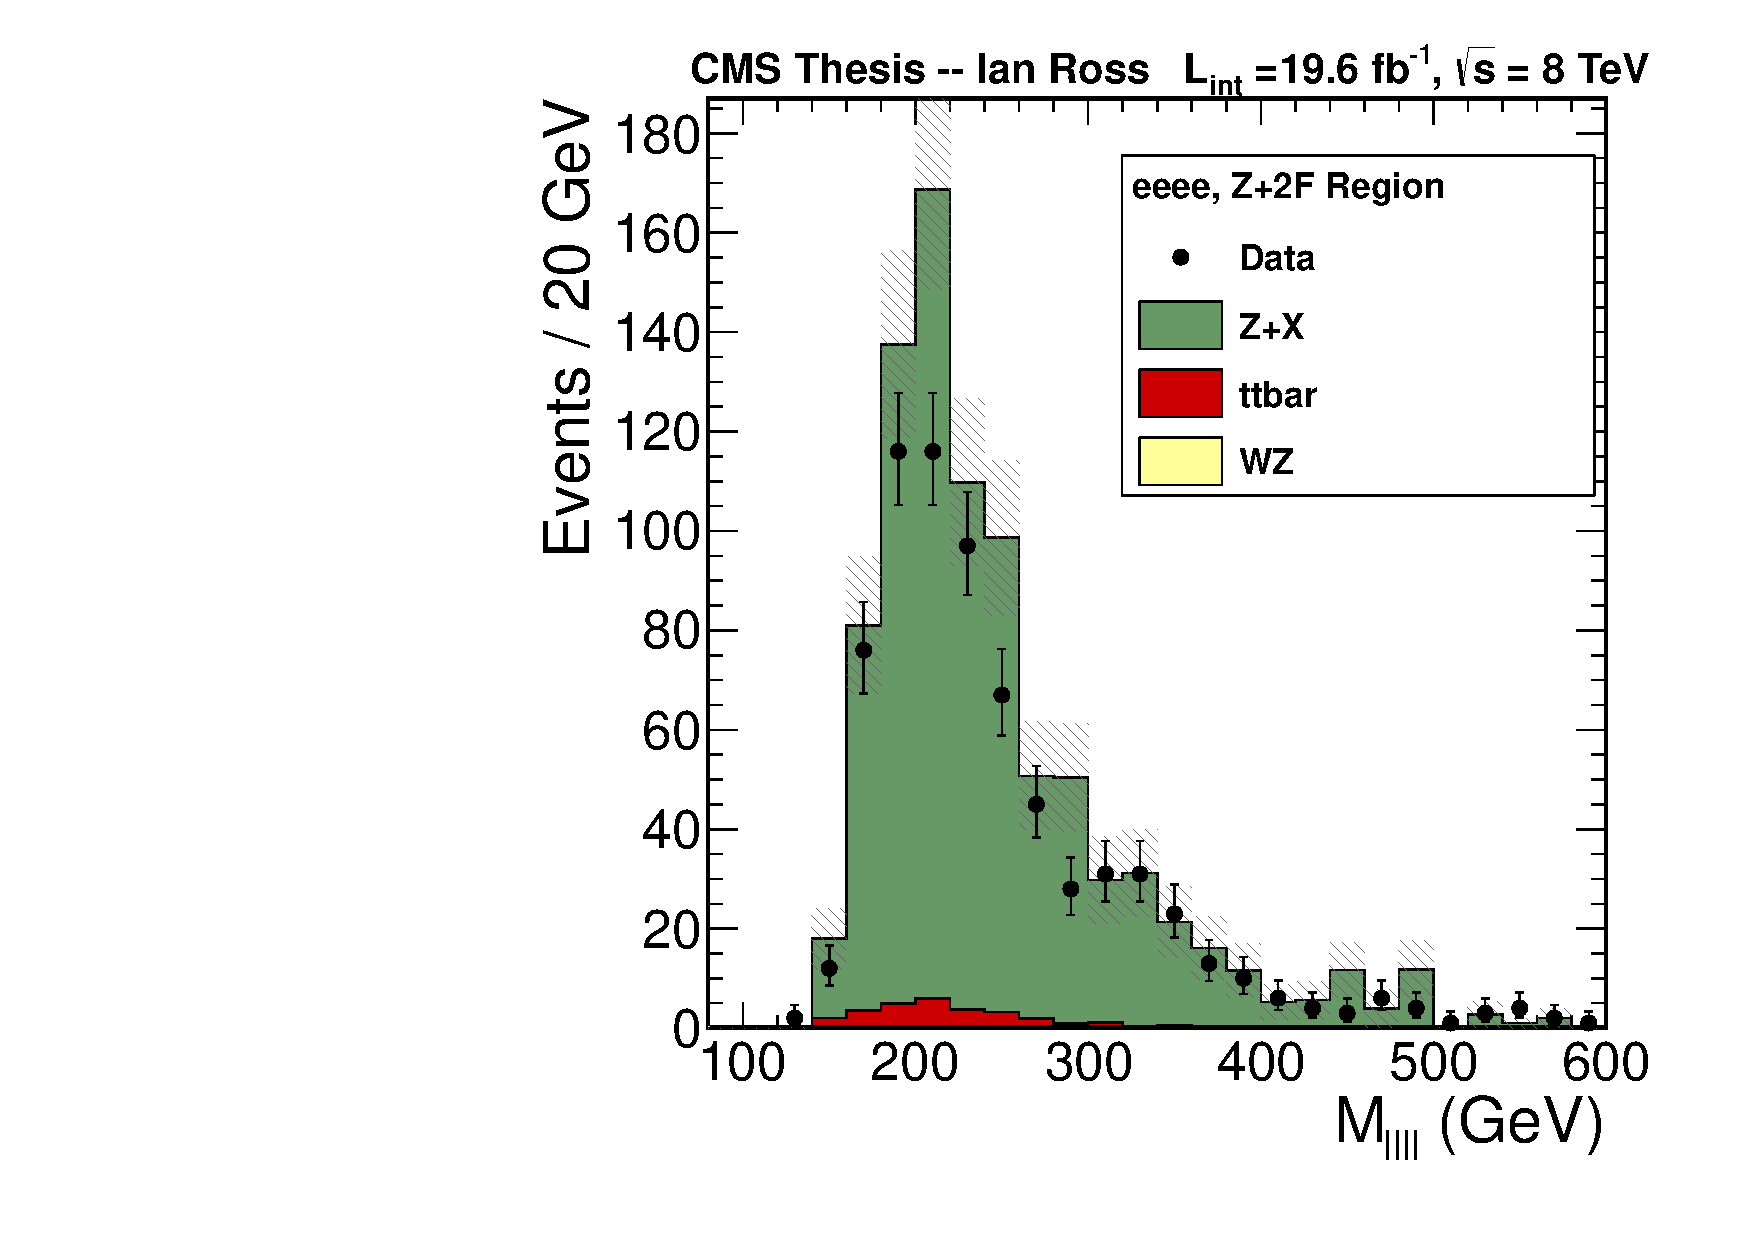
\includegraphics[width=0.45\textwidth]{eeee_AA_highmass}
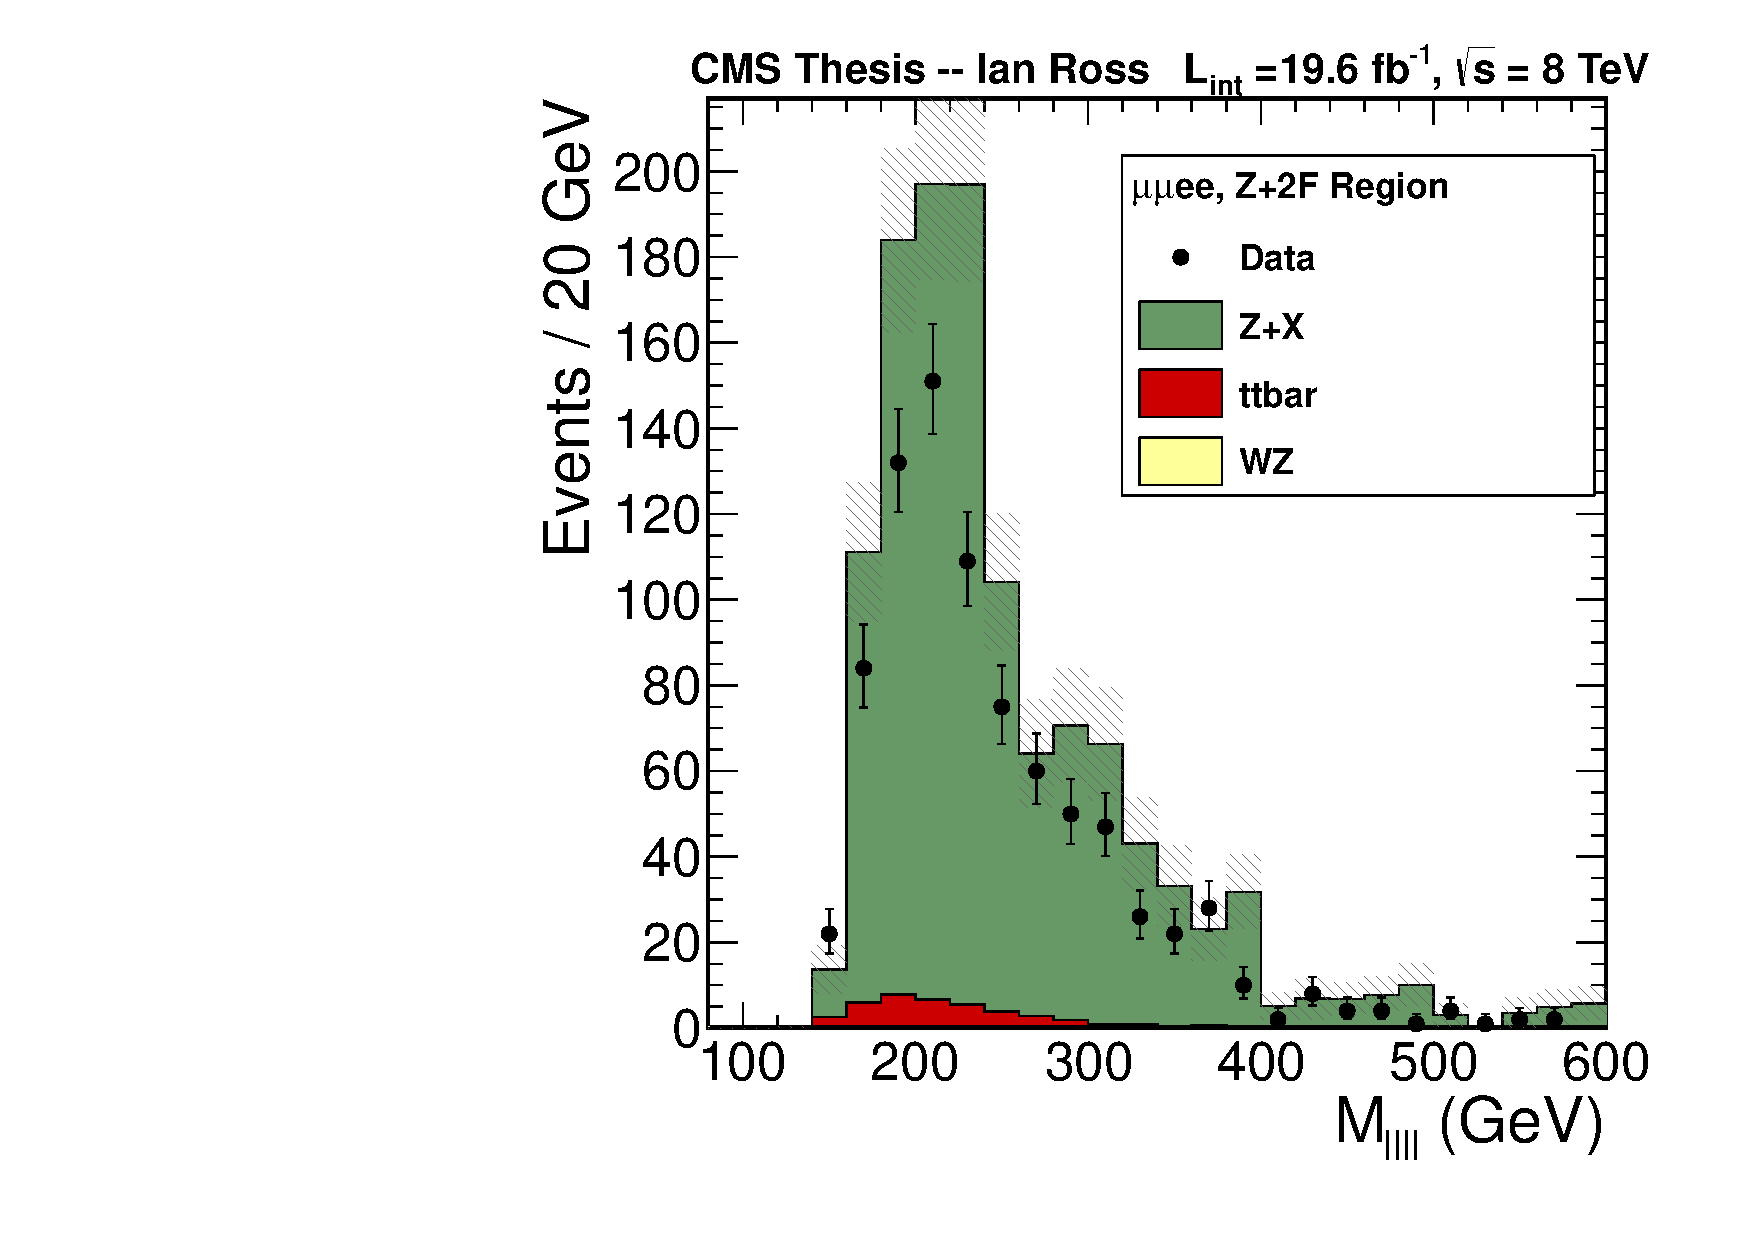
\includegraphics[width=0.45\textwidth]{mmee_AA_highmass}\\
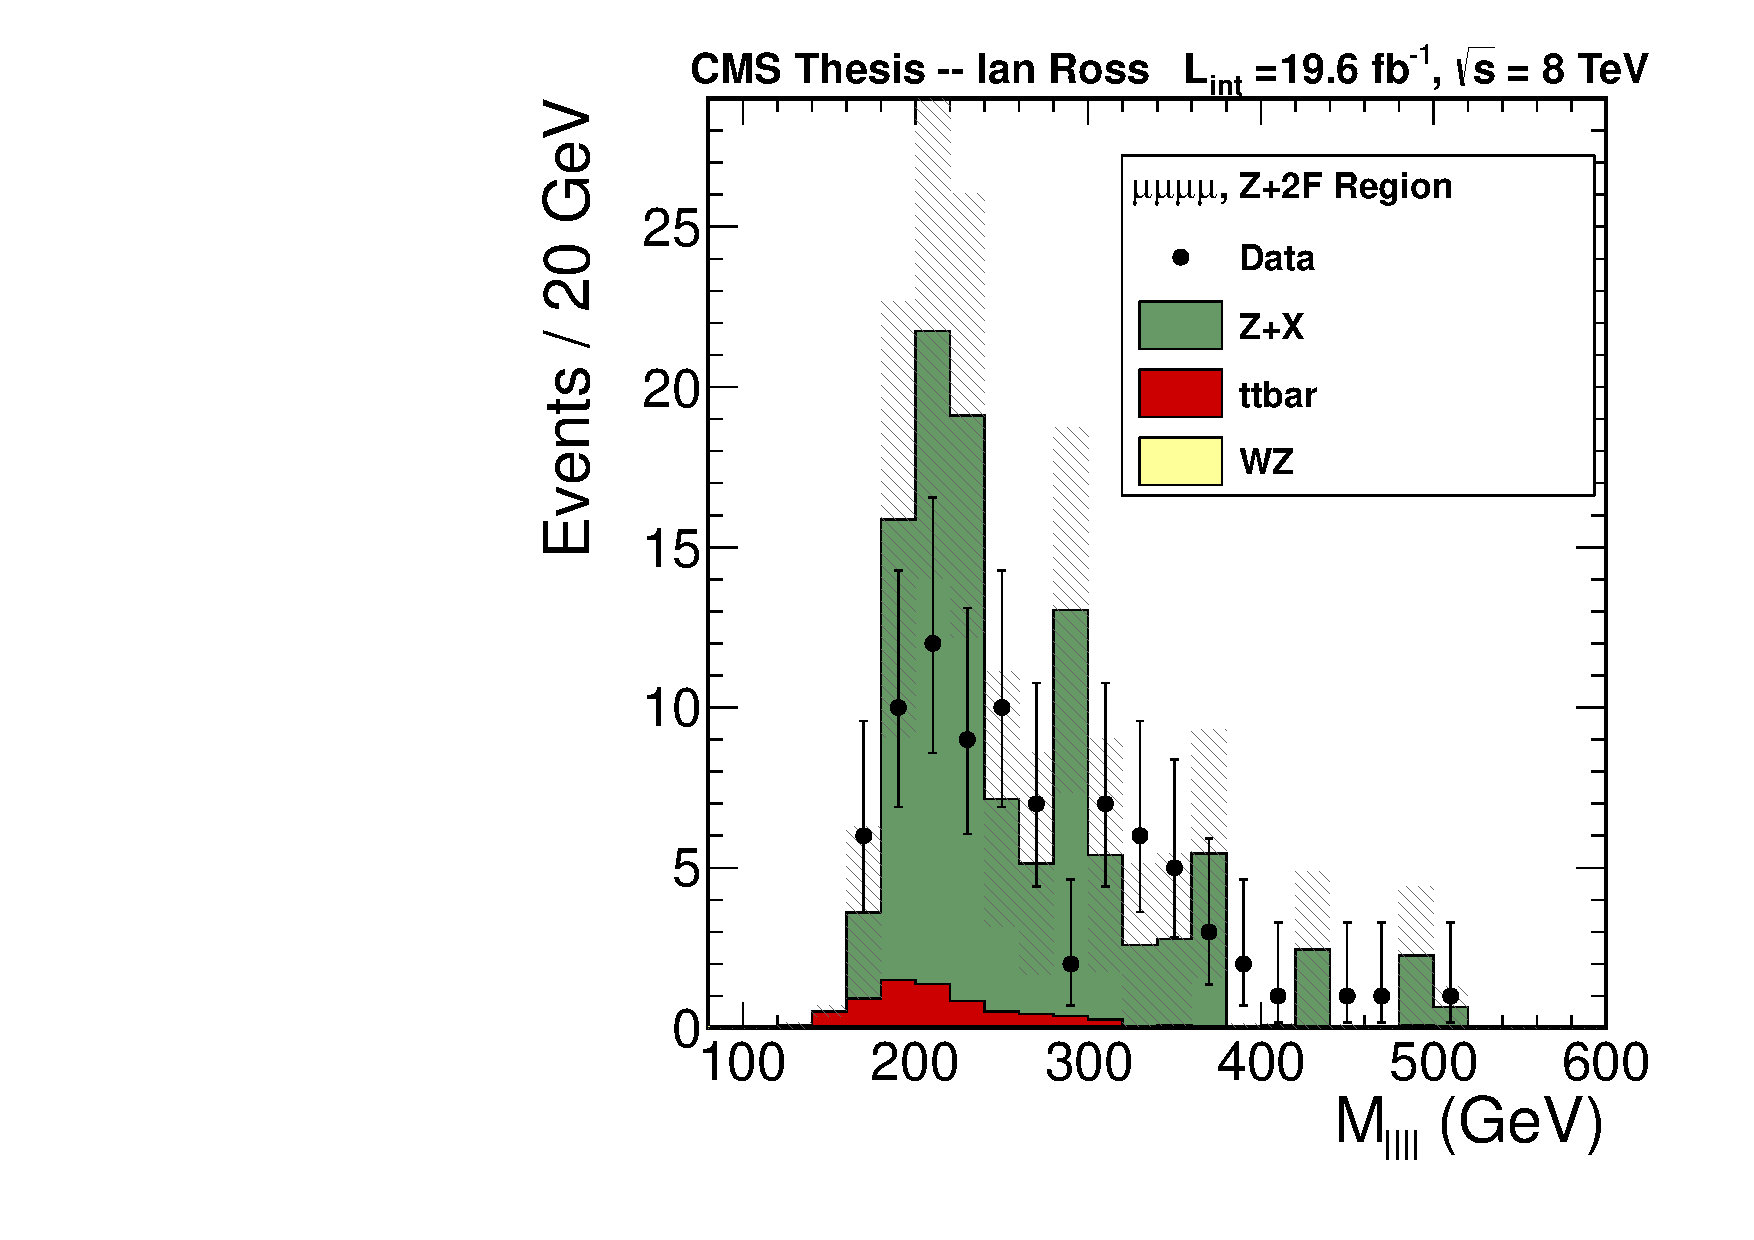
\includegraphics[width=0.45\textwidth]{mmmm_AA_highmass}
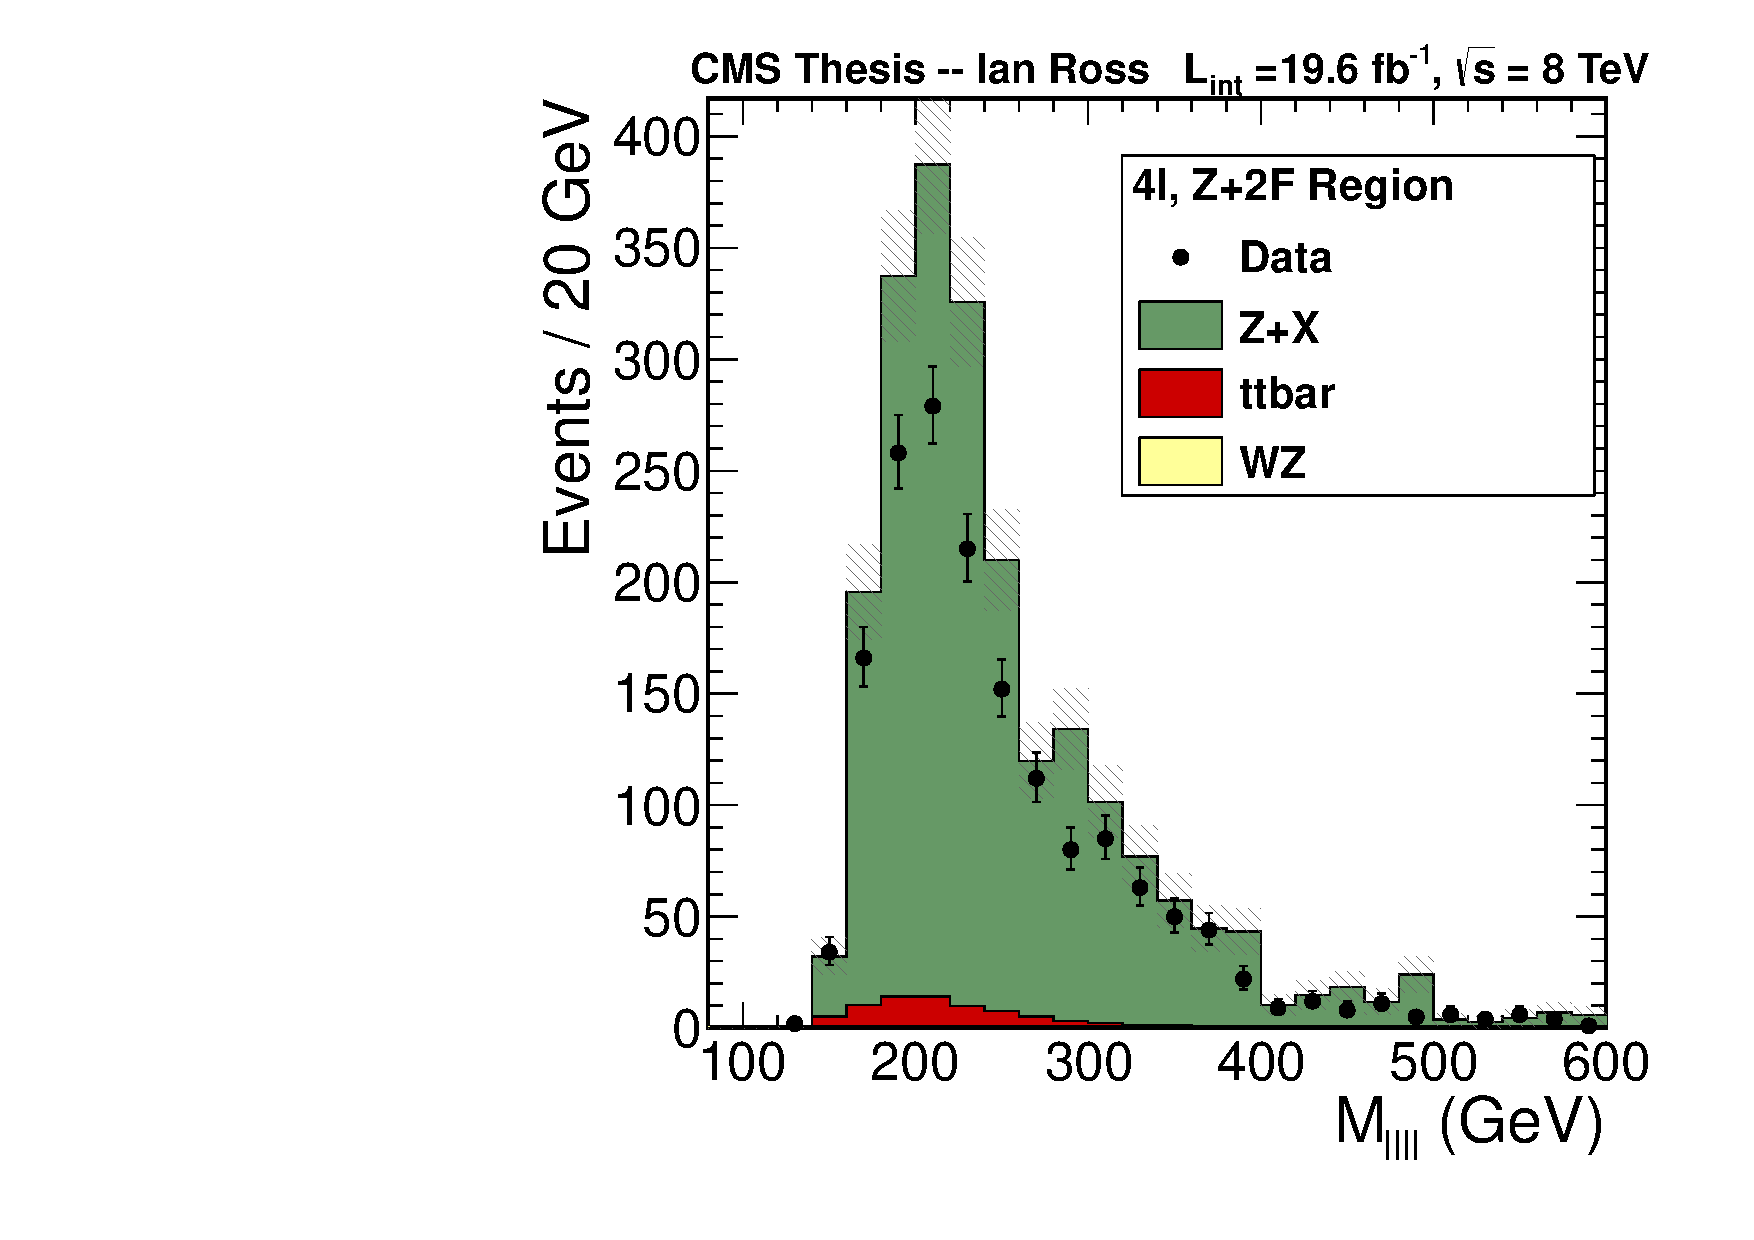
\includegraphics[width=0.45\textwidth]{4l_AA_highmass}\\
\caption[Background estimation region consisting of a \Z plus two failed
leptons, with the high mass requirement.]{Background estimation region consisting of a \Z plus two failed
leptons, with the high mass requirement. Counter clockwise from top right is the eeee, $\mu\mu ee$,
$\mu\mu\mu\mu$, and summed final states.}
\label{fig:AAregions_highmass}
\end{figure}

\begin{figure}[h]
\centering
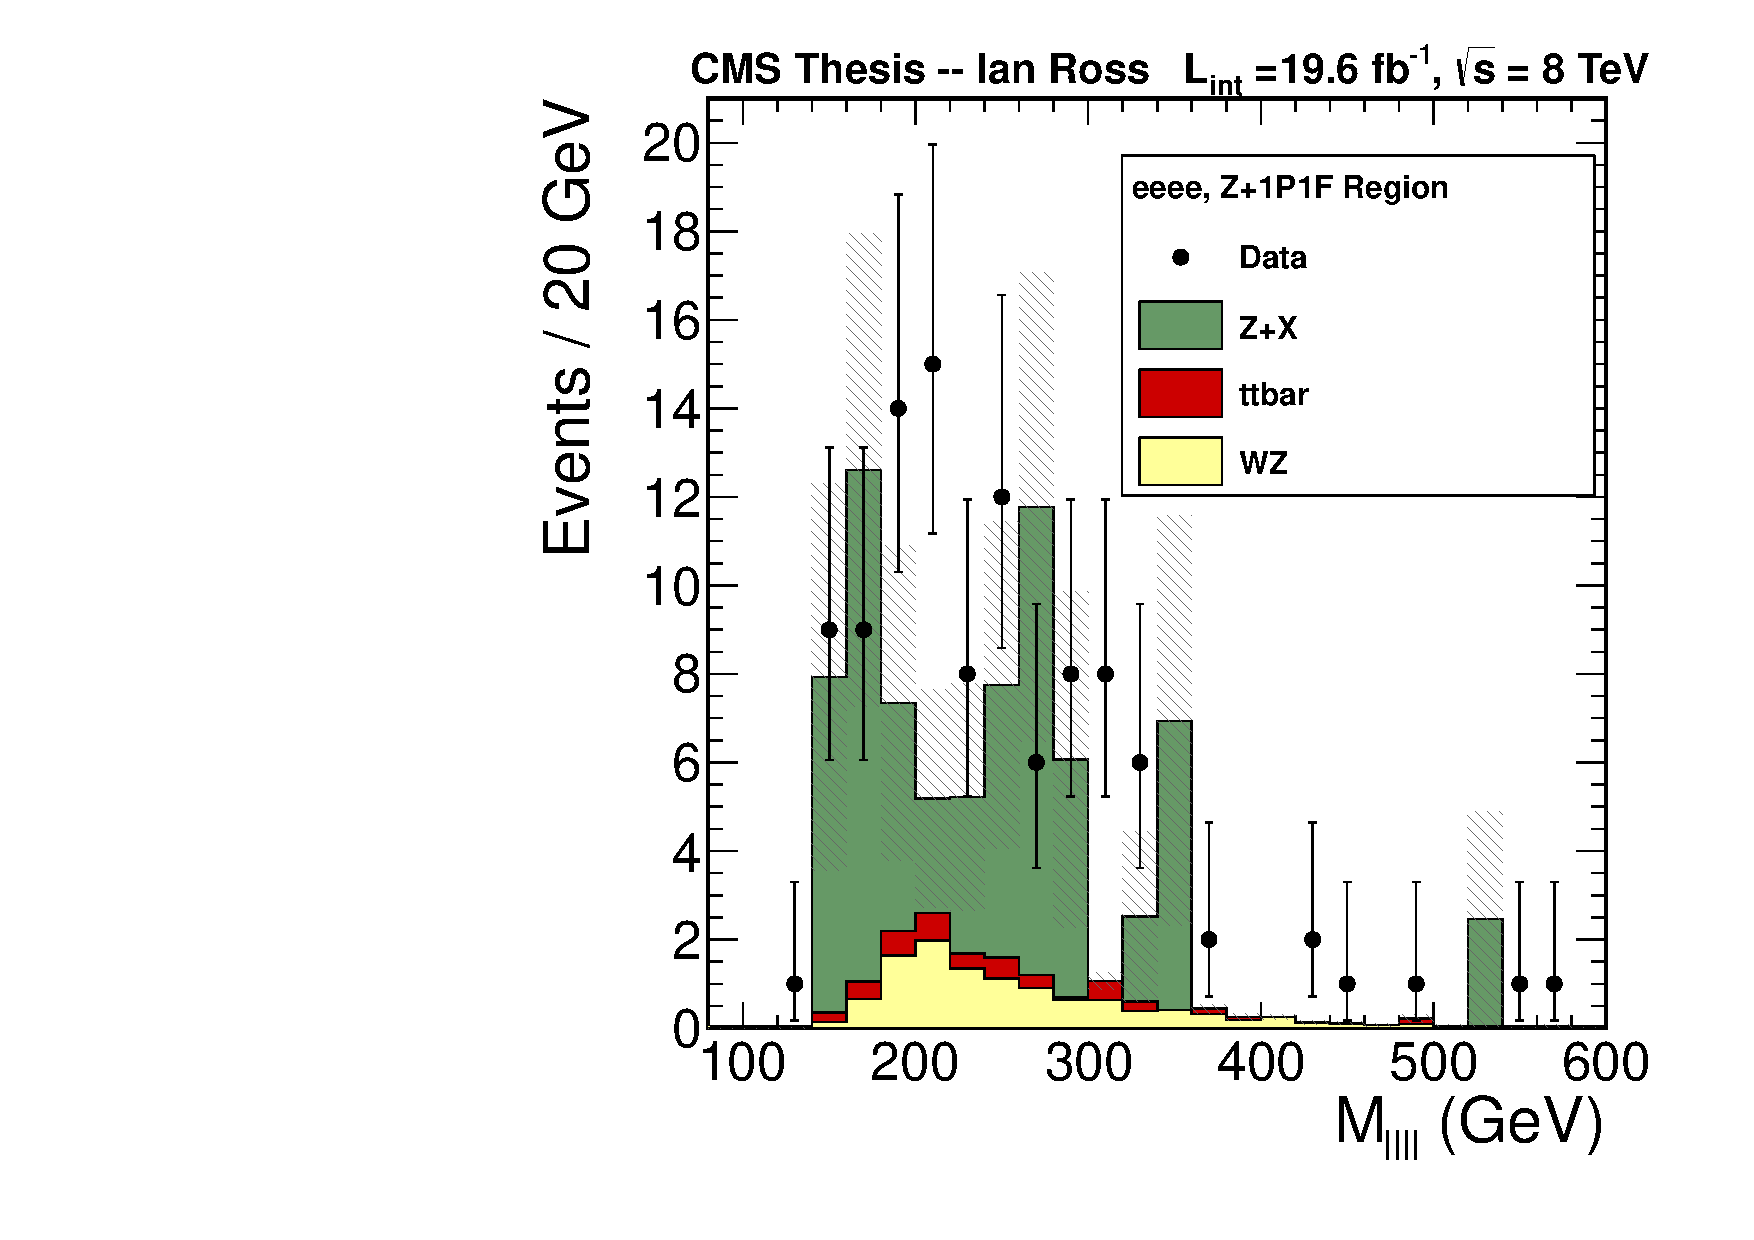
\includegraphics[width=0.45\textwidth]{eeee_IA_highmass}
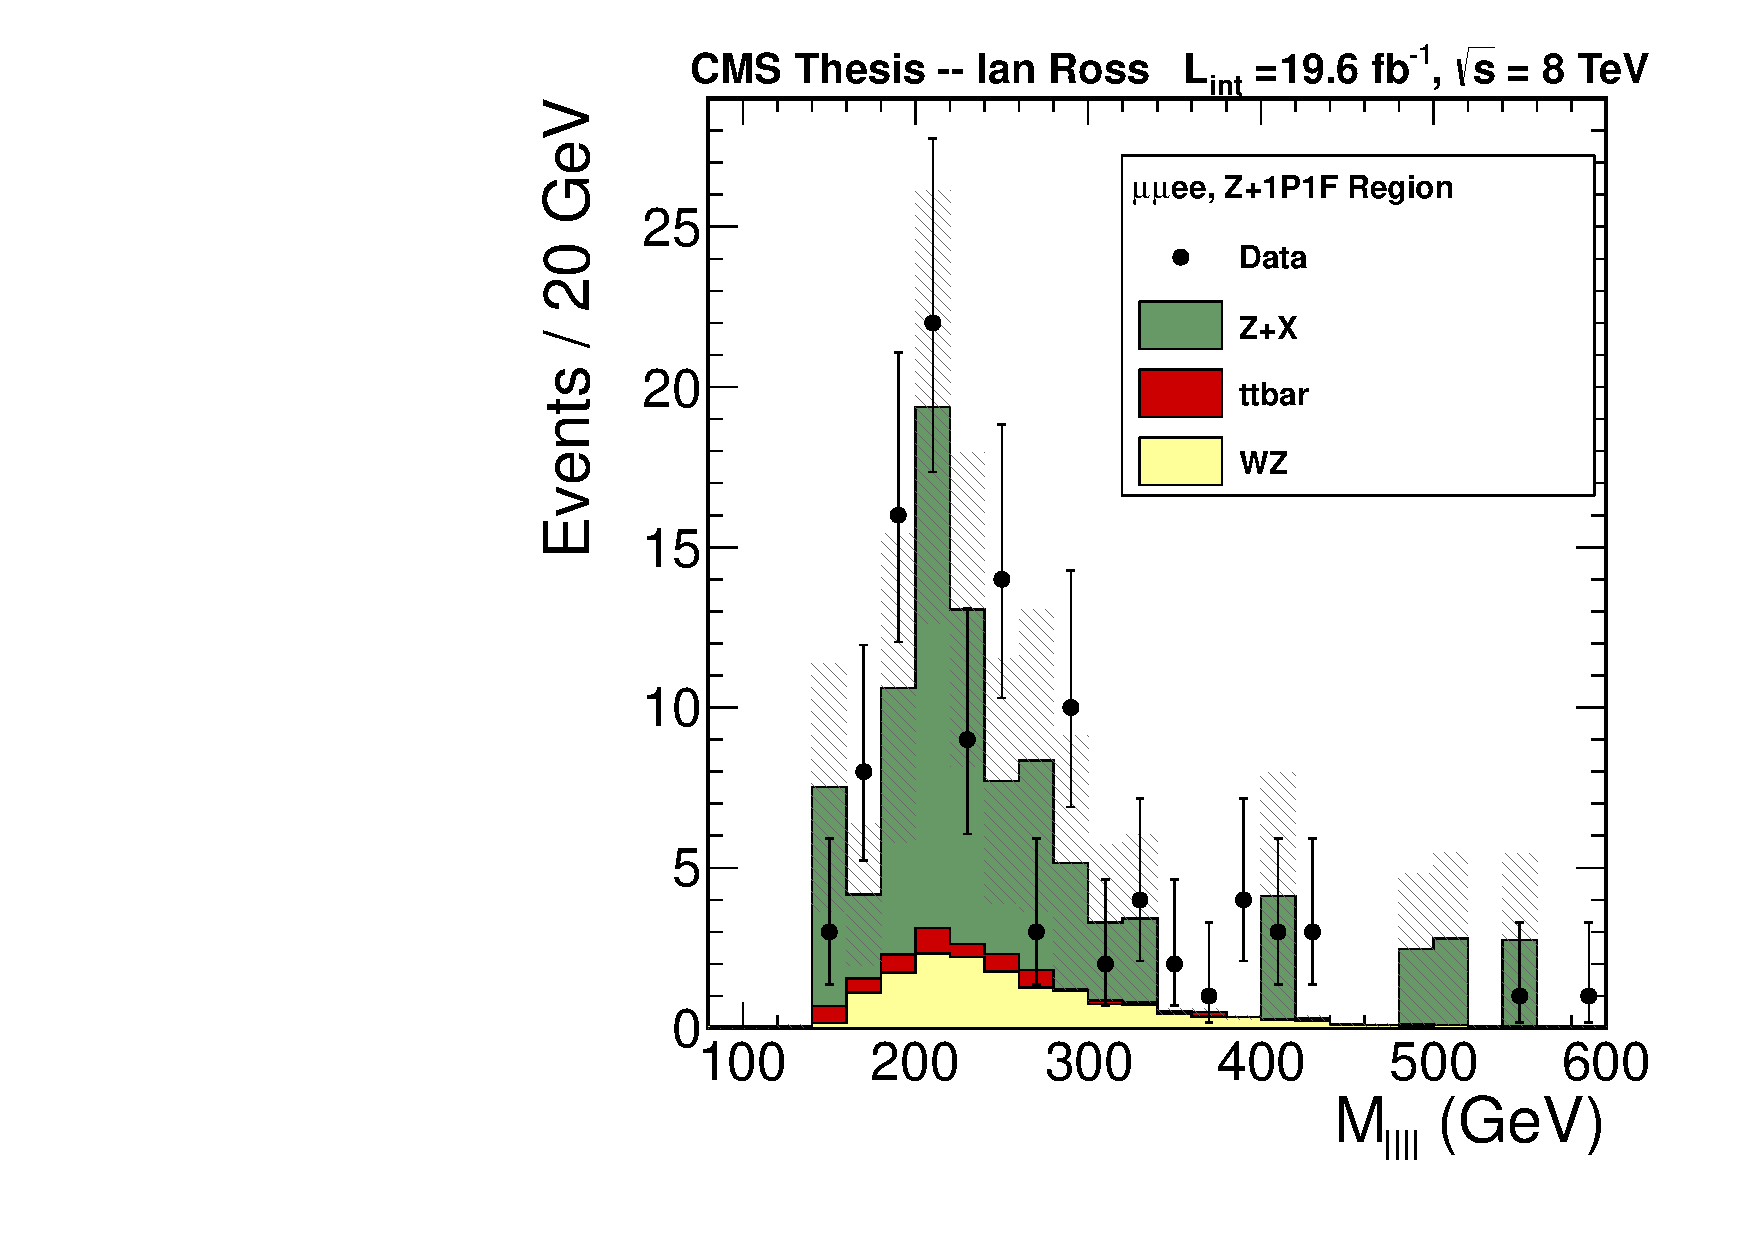
\includegraphics[width=0.45\textwidth]{mmee_IA_highmass}\\
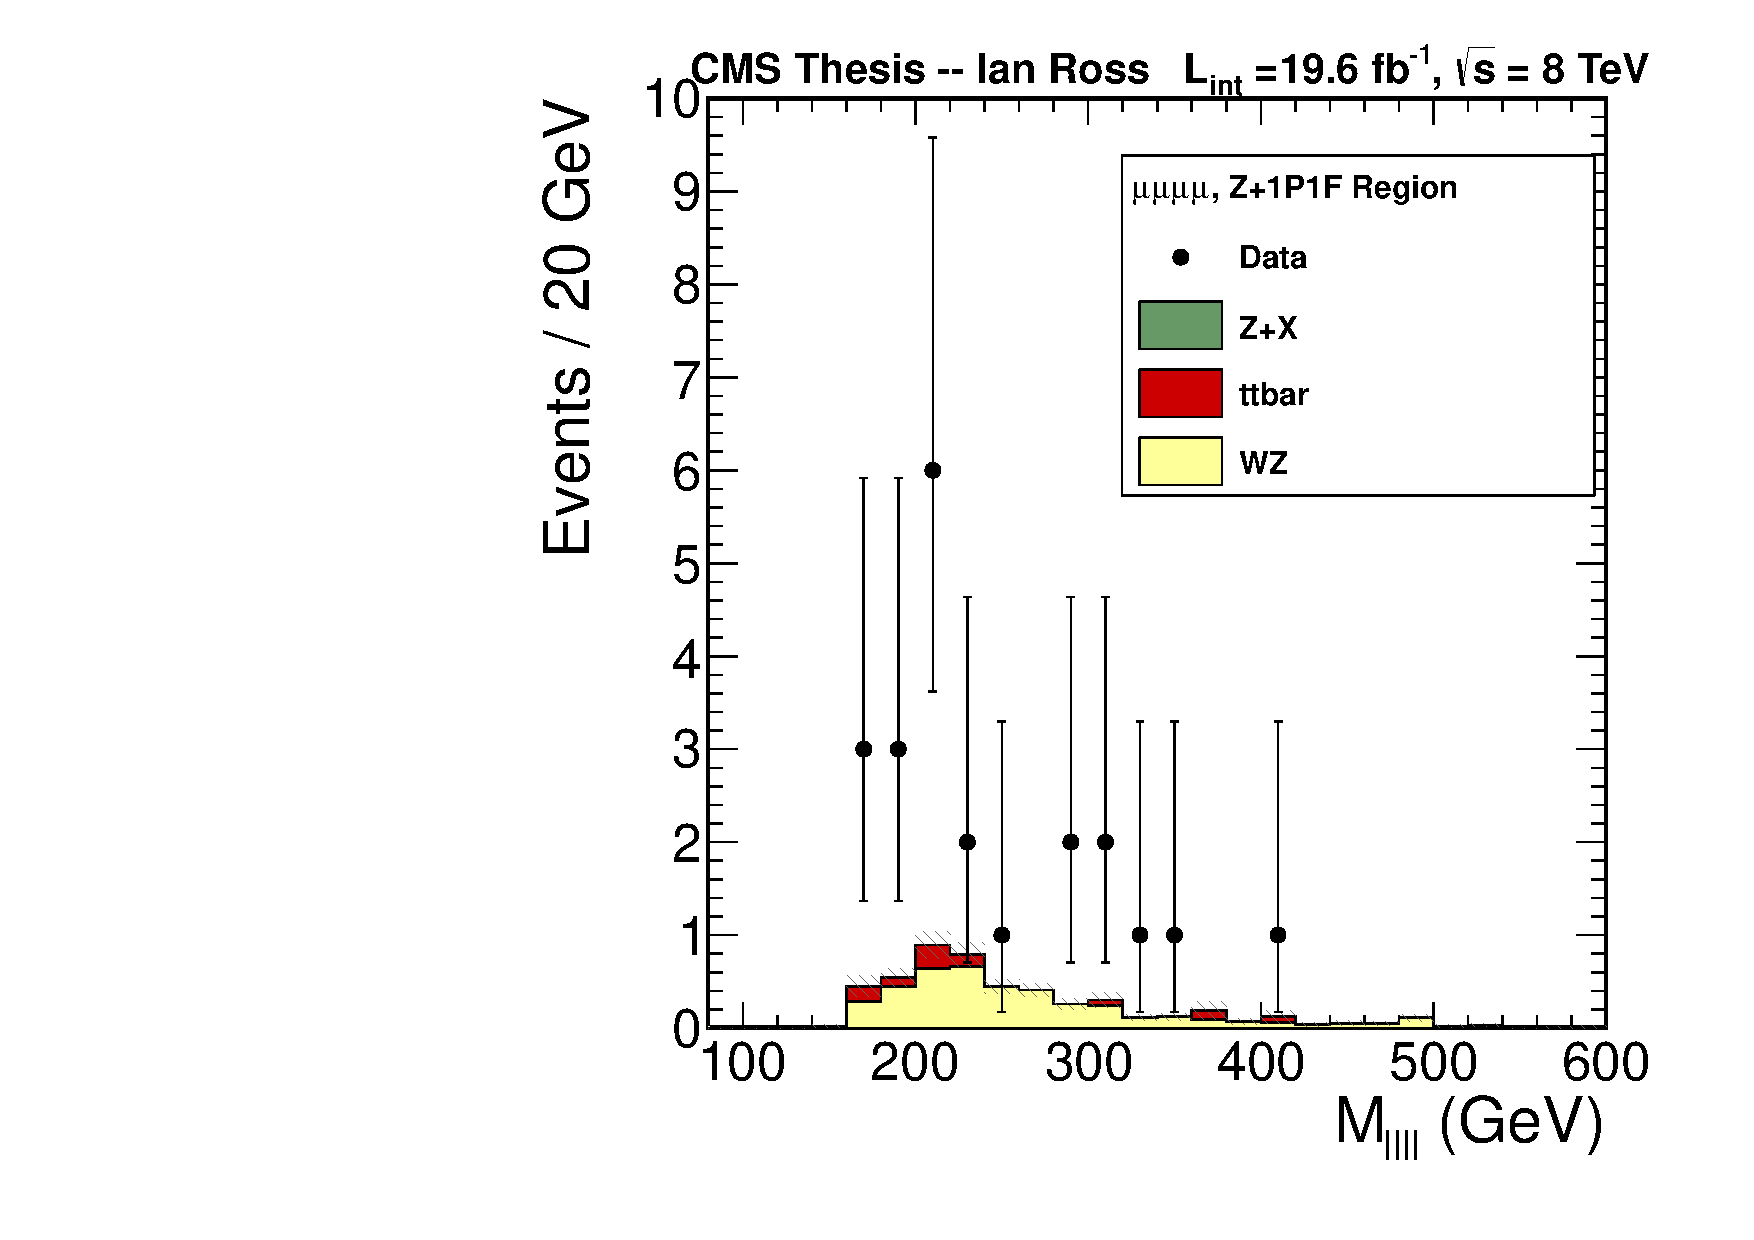
\includegraphics[width=0.45\textwidth]{mmmm_IA_highmass}
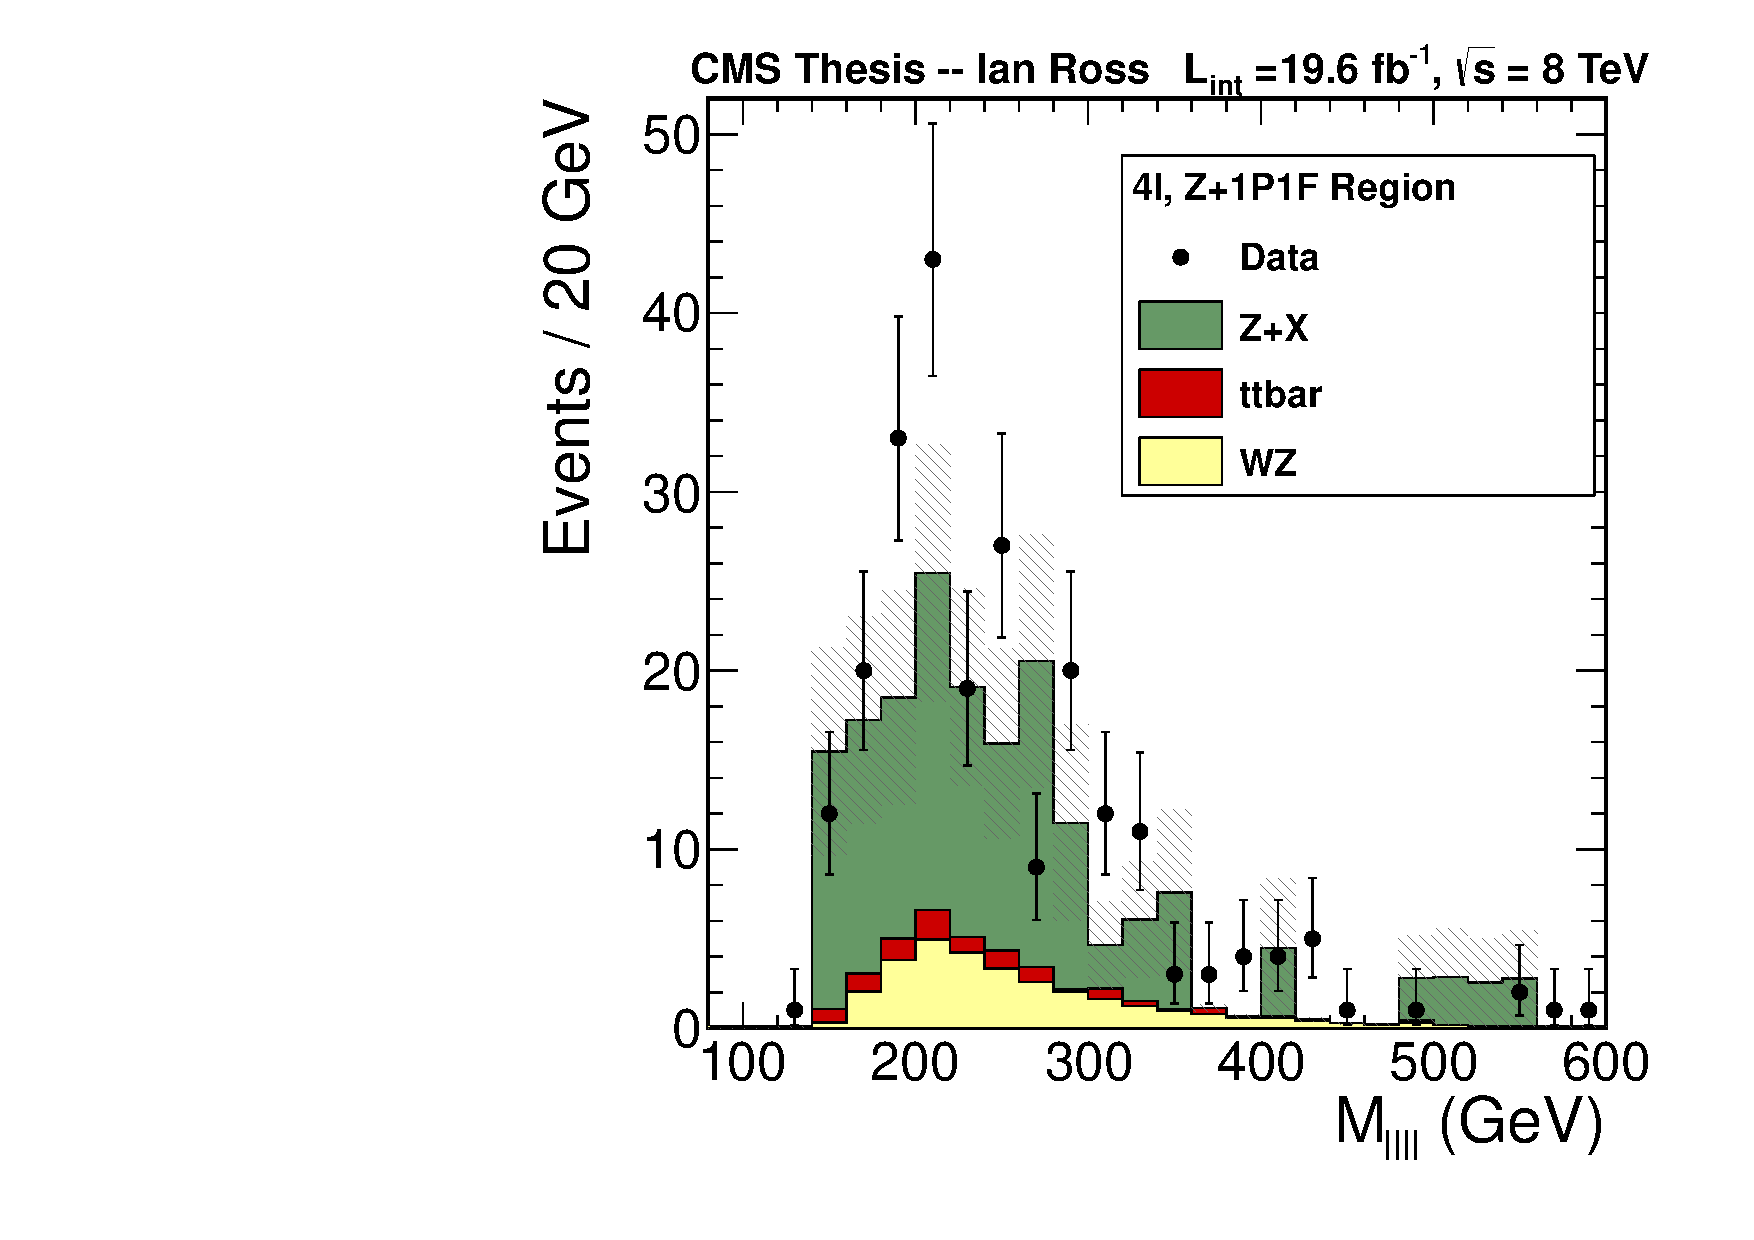
\includegraphics[width=0.45\textwidth]{4l_IA_highmass}\\
\caption[Background estimation region consisting of a \Z plus one passed and one failed
leptons, with the high mass requirement.]{Background estimation region consisting of a \Z plus one passed and
    one failed leptons, with the high mass requirement. Counter clockwise from top right is the eeee, $\mu\mu
    ee$, $\mu\mu\mu\mu$, and summed final states.}
\label{fig:AIregions_highmass}
\end{figure}


In general, $N_F$ background-like events fail the final selection while $N_P$
background-like events pass the final selection, and the fake rate can be written as
\begin{equation}
    f = \frac{N_P}{N_P+N_F} 
\end{equation}
As a result, the population of background events passing the signal selection
can be written as:
\begin{equation}
    \label{eqn:np}
    N_P = N_F \frac{f}{1-f}
\end{equation}

If one assumes the fake rates of Equations~\ref{eqn:fr} and~\ref{eqn:np} are the
same, then the final background is estimated by applying the measured fake rate to
the regions as follows:
\begin{equation*}
    \textrm{Estimated Background} = \frac{f}{1-f}
    N_{\textrm{1P1F}} - \frac{f^2}{(1-f)^2} N_{\textrm{2F}}
\end{equation*}
where $N_{\textrm{1P1F}}$ is the number of events in the Z+1P1F region, with the
MC-driven expectation of ZZ contamination removed and $N_{\textrm{2F}}$ is the
Z+2F equivalent. The removal of the Z+2F contribution is required due to the
fact that these events are doubly represented in the Z+1P1F region, as the
population here already contains Z+2jet events that underwent a $2 \choose 1$
migration, as there are two selected lepton `slots' for a jet to fake. The flow
of these events is diagrammed in~\ref{fig:bgFlow}. 

\begin{figure}[h]
\centering
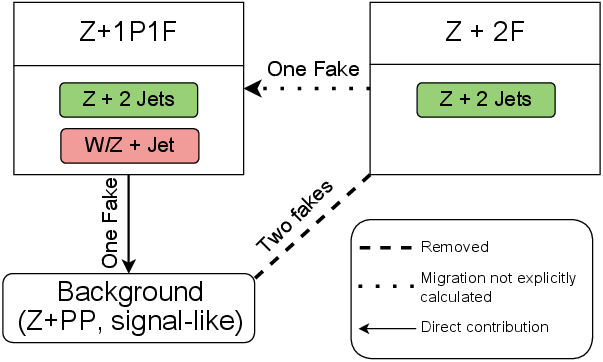
\includegraphics[width=0.80\textwidth]{bgFlow2Cat}
\caption[Diagram depicting the flow of events in the reducible background
estimate.]{Diagram depicting the flow of events in the reducible background. A
dotted line indicated a migration that does not explicitly enter the background
estimate, a solid line indicates a positive net contribution, while a dashed
line indicates a removal from the estimate. The ``P'' and ``F'' stand for
additional loose leptons which pass or fail final selections, respectively.}
\label{fig:bgFlow}
\end{figure}

\section{Final State Radiation Recovery}
It is possible for electrons and muons produced in a Z boson decay to radiate a
photon, resulting in a $Z\rightarrow \ell \ell \gamma$ final state. Because the
photons are emitted along an almost equal trajectory, the electron
reconstruction process often captures these additional photons. However, it is
possible that the electron reconstruction misses the radiated photons and, in
addition, no such recovery is inherent to the muons. Given the criticality of
precise mass measurements, a final state radiation (FSR) recovery algorithm is
implemented in order to fully reconstruct the four-momentum of the Z candidates. 

The FSR recovery begins by first defining a set of FSR-candidate photons. To
start, a collection of photons is built from the Particle Flow photon
collection. In addition, photon candidates are built from the electromagnetic
calorimeter deposits near Particle Flow muons. The photons are required to have
$p_T > 2$~GeV, within $|\eta|$ of 2.4, and be well separated from the
superclusters of any electrons passing the $p_T$, identification, and vertex
compatibility requirements ($\Delta R > 0.15$, $\Delta \phi > 2$, and $\Delta
\eta > 0.05$).  The isolation for these photons is then computed, using a cone
size of $\Delta R < 0.3$, with thresholds of 0.2 and 0.5~GeV on the charged and
neutral+photon components. 

For each photon, the nearest lepton from the Z candidate is found. If the photon
is co-linear with the lepton ($\Delta R(\ell \gamma) < 0.015$, then the photon is
kept. If the separation between the photon and lepton is wider ($\Delta R(\ell
\gamma) < 0.5$), then the photon is kept if its $p_T$ is above 4~GeV and its
relative isolation is less than 1.

Finally, the list of FSR candidate photons is considered with the Z candidate
objects.  It is important to note that these Z candidates are built from leptons
with the isolation criteria not yet applied, as the FSR photon's removal from
the leptons' isolation can cause them to migrate from failing to passing the
selection.  With the four-momenta of the photon summed to that of the Z
candidate, the photon is considered to be a successful recovery if:
\begin{itemize}
    \item $| M_{\ell \ell \gamma} - M_{\Z} | < | M_{\ell \ell} - M_{\Z} | $
    \item $4 < M_{\ell \ell \gamma} < 100~GeV$
\end{itemize}
If these criteria are met, then the photon is removed from that Z candidate's
leptons' isolation cones and the Z ($\rightarrow \ell \ell \gamma$) object is
considered to as the Z candidate.

The effects of the FSR recovery can be seen on simulated $\Z \rightarrow ee$ and $\Z
\rightarrow \mu \mu$ peaks in Figure~\ref{fig:fsrRecovery}. 

\begin{figure}[h]
\centering
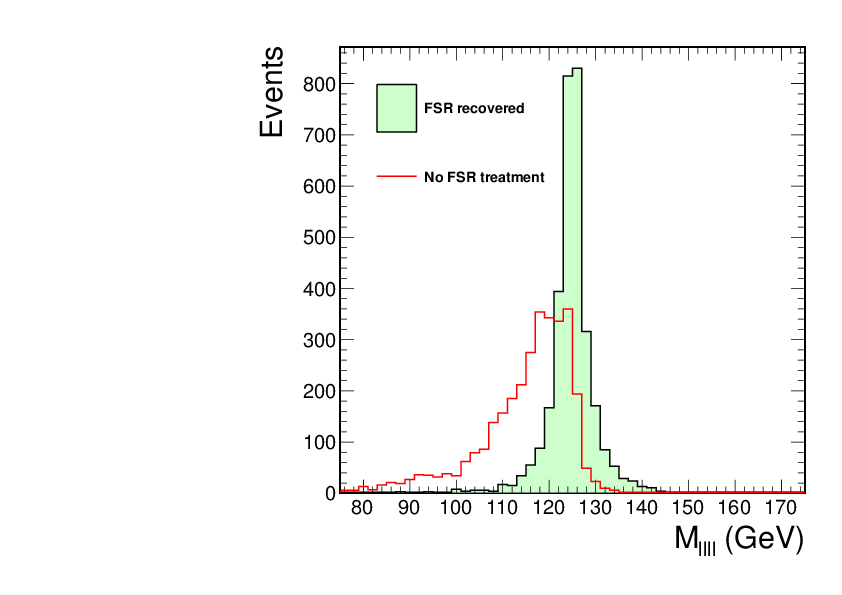
\includegraphics[width=0.50\textwidth]{recovered_fsr}
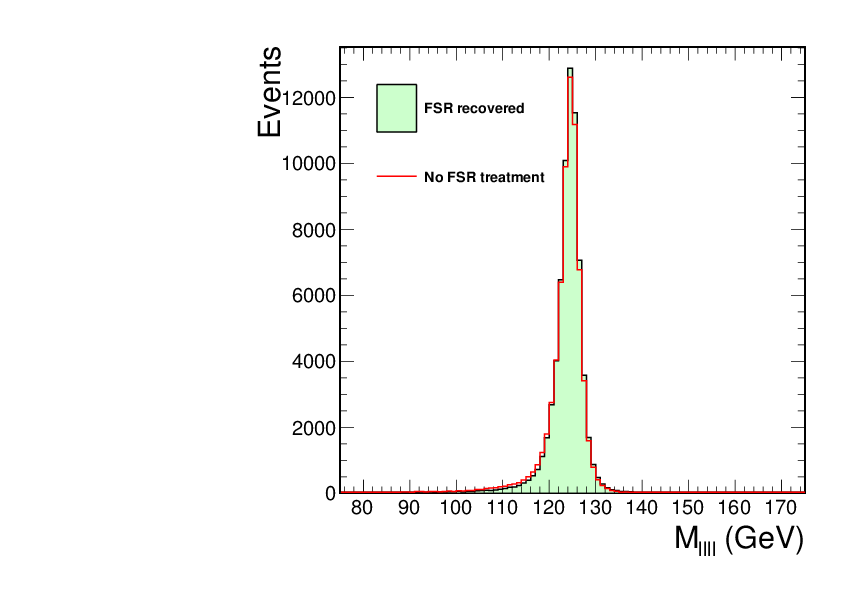
\includegraphics[width=0.50\textwidth]{recovered_fsr_all}
\caption[A simulated $H\rightarrow2e2\mu$ ($m_H = 125 GeV$) peak, with and without FSR
recovery.]{A simulated $H\rightarrow2e2\mu$ ($m_H = 125 GeV$) peak, with and without the
    FSR recovery. The FSR recover effects only a fraction (~6\% total, top) of the
    events, but the overall effect (bottom) is a few percent gain in resolution.
}
\label{fig:fsrRecovery}
\end{figure}

\section{Kinematic Discriminant}
A kinematic discriminant is introduced in order to utilize the angular
differences between $H\rightarrow ZZ \rightarrow \ell\ell\ell\ell$ and $ZZ
\rightarrow \ell\ell\ell\ell$ decays. Five angles define the angular system in
the ZZ rest frame (as pictured in diagram~\ref{fig:angles}:
\begin{itemize}
    \item $\theta_1$ and $\theta_2$, the helicity angles defined in each Z's
        rest frame.
    \item $\theta\ast$, the production angle of the Z boson with respect to the
        beam axis
    \item $\Phi_1$, the azimuthal angle between the Z1 decay plane and the Z
        production plane
    \item $\Phi$, the angle between the Z1 and Z2 decay planes
\end{itemize}

The probability that a Higgs (or ZZ) candidate was created with invariant Z
masses $M_{Z1}$ and $M_{Z2}$ and an angular system defined by the angles $\vec
\Omega$ are proportional to their respective elements:
\begin{equation}
    P_{signal} (M_{Z1}, M_{Z2}, \vec \Omega | M_{\ell\ell\ell\ell} ) = |
    ME_{signal} |^2
\end{equation}
\begin{equation}
    P_{bkg} (M_{Z1}, M_{Z2}, \vec \Omega | M_{\ell\ell\ell\ell} ) = |
    ME_{bkg} |^2
\end{equation}
A kinematic discriminant can be built to classify events as more or less
signal-like:
\begin{equation}
    KD = \frac{P_{signal}}{P_{signal}+c\cdot P_{bkg}} = \left(1+\frac{c\cdot
    P_{bkg}}{P_{signal}} \right)^{-1}
\end{equation}
This gives a continuously varying discriminant, with background-like events
pushed toward 0 and signal-like events near 1.
$P_{bkg}$ is evaluated using MCFM~\cite{MCFM}, while JHUGen~\cite{spin} is used to train
the signal samples.

\begin{figure}[h]
\centering
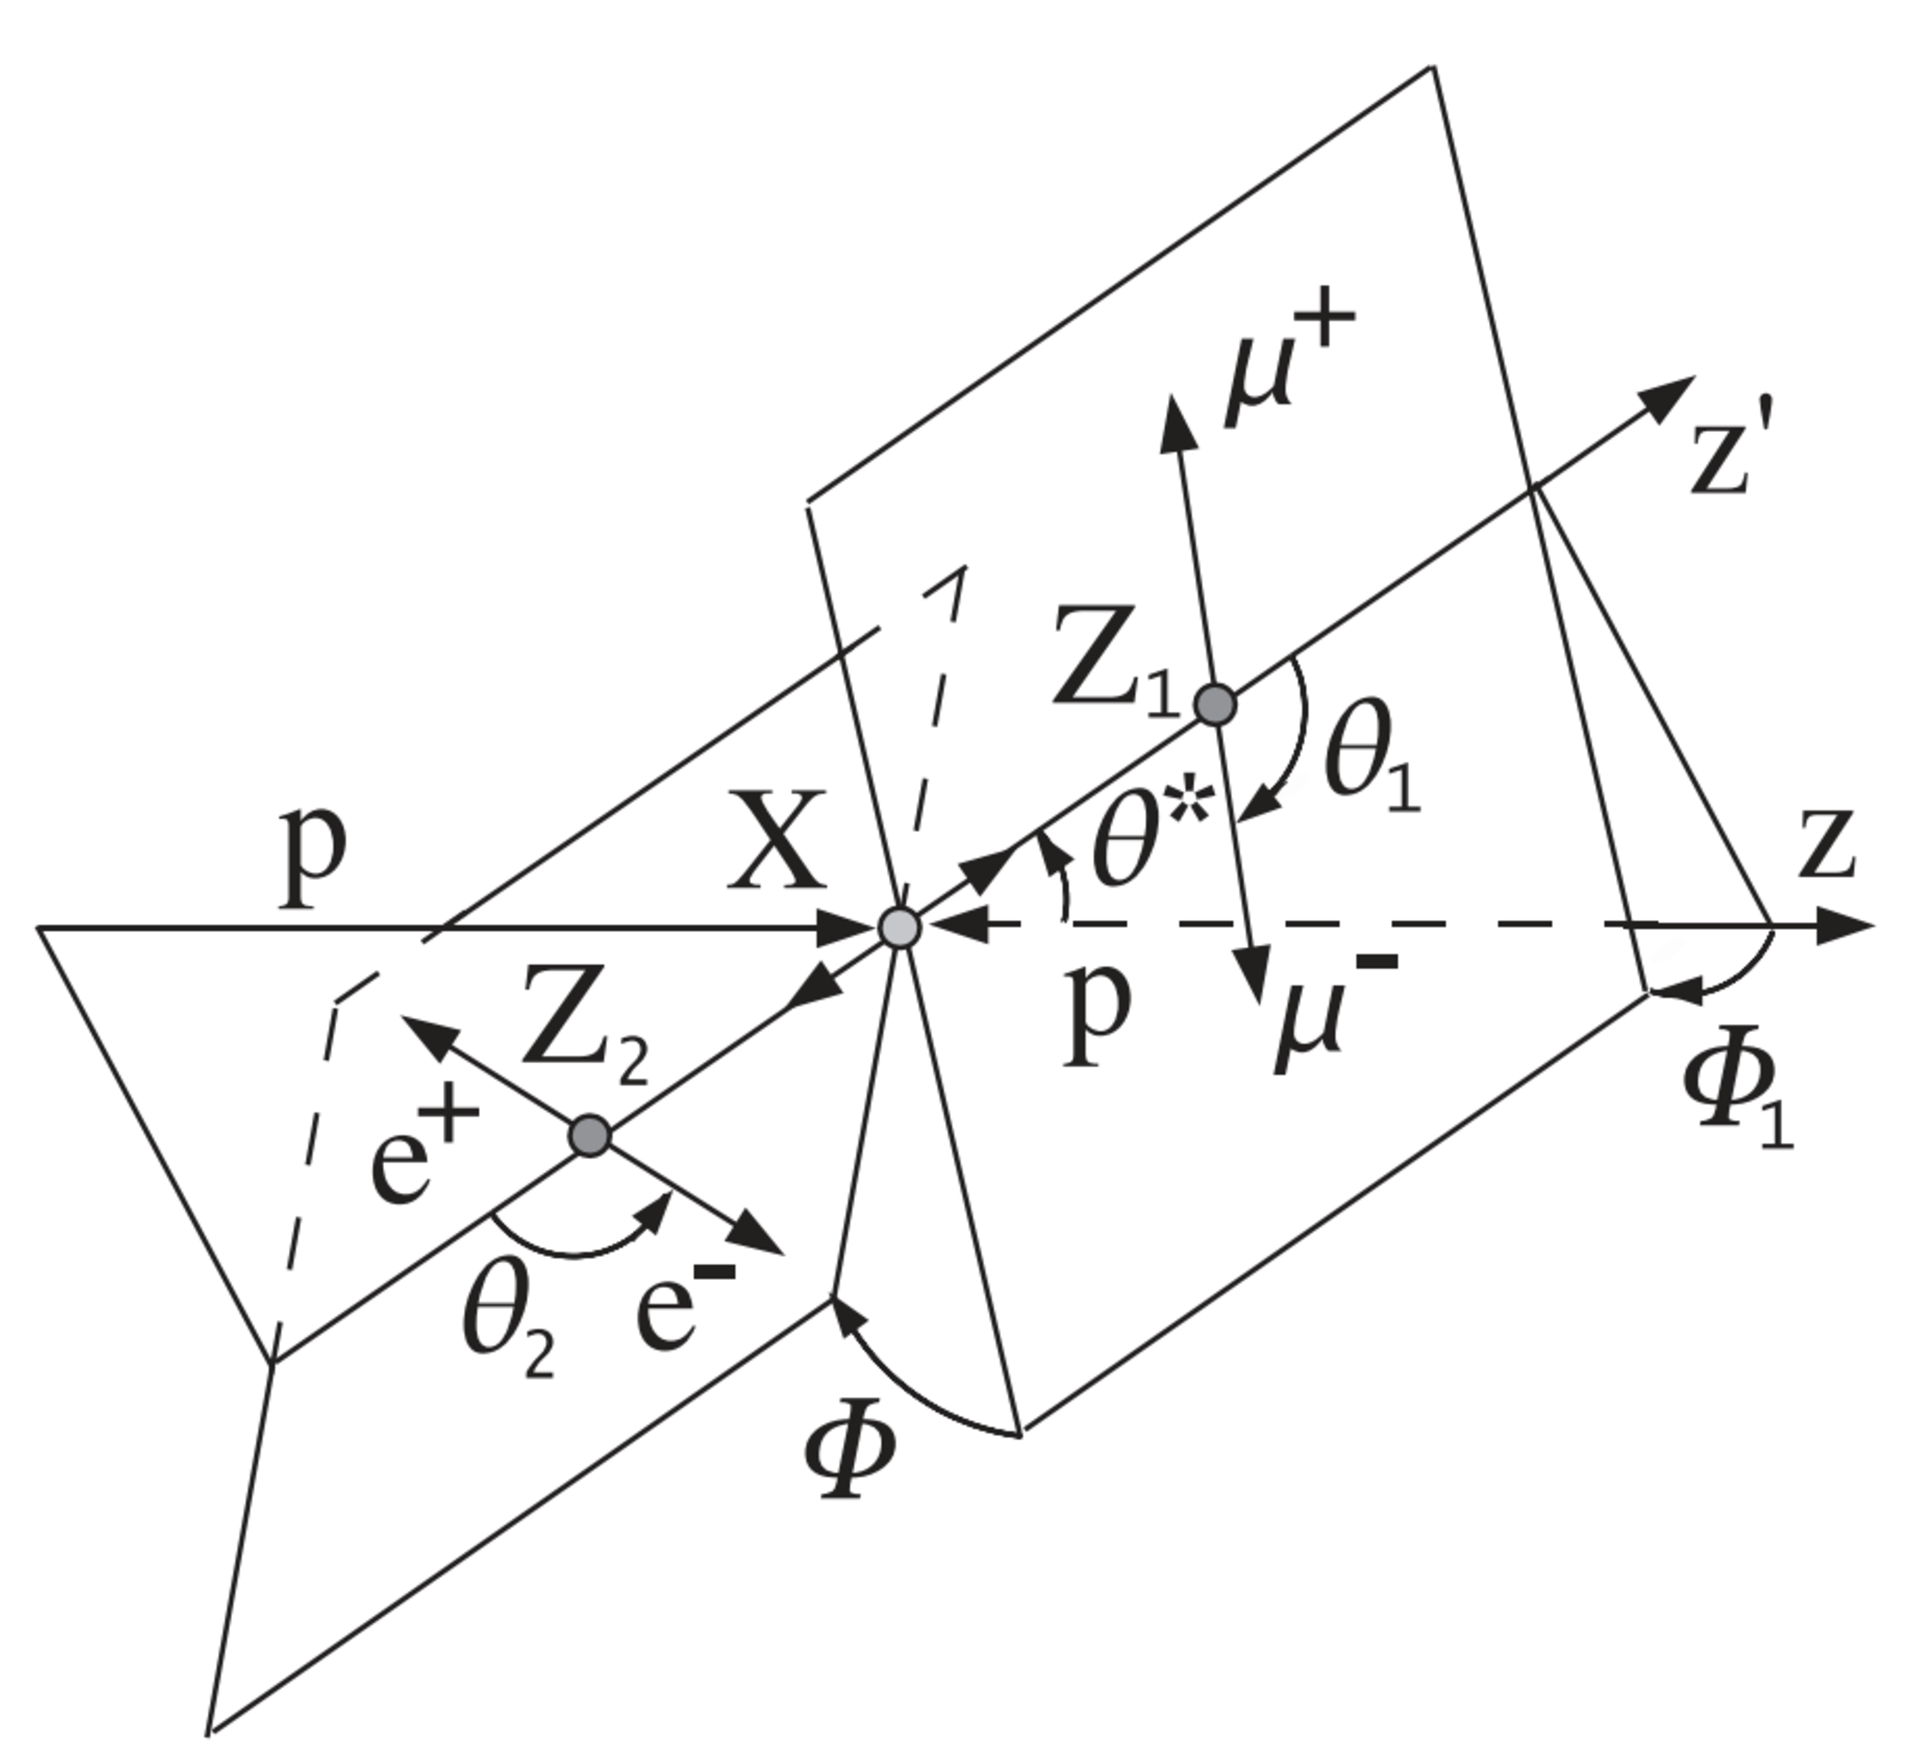
\includegraphics[width=0.60\textwidth]{angles}
\caption[The angular definitions in the ZZ rest frame.]{The angular definitions
in the ZZ rest frame.}
\label{fig:angles}
\end{figure}

\section{Final event selection}
In order to build the final physics events, the selected leptons must be
combined into composite Z candidates, which in term are combined into the final
ZZ system. This is done by first combining same-flavor (SF), opposite sign leptons
(which pass all identification criteria) into an initial Z candidate. Then the
remaining leptons (which pass the loose criteria defined above) are combined
into same-flavor combinations. All possible combinations of Z candidate plus SF
combinations are stored from the events, allowing easy access to both
signal-like events (in which the second candidate passes the tighter criteria
are are of opposite sign) and background-like events (in which the second pair
of leptons fail the tighter selection and/or are of the same sign). 

For both of these sets of Z candidates (both those explicitly passing
identification and those that have no restrictions), the FSR recovery is run.
This allows the effects of the FSR state recovery to be properly accounted for
in both signal and background-like candidates. 

After the FSR recovery, the isolation requirements are placed onto the first Z
candidate. Then, selection criteria are applied onto the second Z candidate,
sorting the ZZ candidates into signal, Z+1P1F, or Z+2F regions (for both SS and OS
secondary pairs).

\subsection{Candidate combinatorics and arbitration}
In the $eeee$ and $\mu\mu\mu\mu$ final states, the ways in which to
combine the opposite-sign, same flavor pairs is ambiguous. Additionally, it is
possible that more than four good leptons exist, allowing multiple ZZ candidates
to exist within an event. 
This effect, plus the asymmetric mass selections, on the Z candidates means that
some arbitration must be applied. The simplest arbitration is the ``best Z
mass'' selection, in which the $Z_1$ is defined to be the pair whose invariant
mass is closest to the nominal Z mass. Then, from the remaining possible $Z_2$
candidates, the one with the highest scalar sum of lepton $p_T$s is chosen.

The background regions are treated differently. Because each of the candidates
represents a possible migration into the signal region, all unique combinations
are kept. 

\subsection{Signal selection}
This analysis considers two separate set of criteria in its two separate
searches. The two criteria differ only in the criteria placed on the invariant
masses of the Z candidates.
The Higgs search necessitates picking up $Z\gamma*$ contributions, so a wider
invariant mass range is allowed:
\begin{equation*}
40 < M_{Z_1} < 120 GeV
\end{equation*}
\begin{equation}
12 < M_{Z_2} < 120 GeV
\label{eqn:lowmass}
\end{equation}

In the measurements pertaining to the anomalous triple gauge couplings and
ZZ differential cross sections, both \Z bosons are required to be on-shell,
eliminating the contributions from $\gamma *$ production:

\begin{equation*}
60 < M_{Z_1} < 120 GeV
\end{equation*}
\begin{equation}
60 < M_{Z_2} < 120 GeV
\label{eqn:highmass}
\end{equation}
The Higgs search (the so-called low-mass criteria) and the Standard Model/triple
gauge coupling measurements (the high-mass criteria) differ only in the mass
requirements listed in equations~\ref{eqn:lowmass} and~\ref{eqn:highmass}.

\begin{figure}[h]
\centering
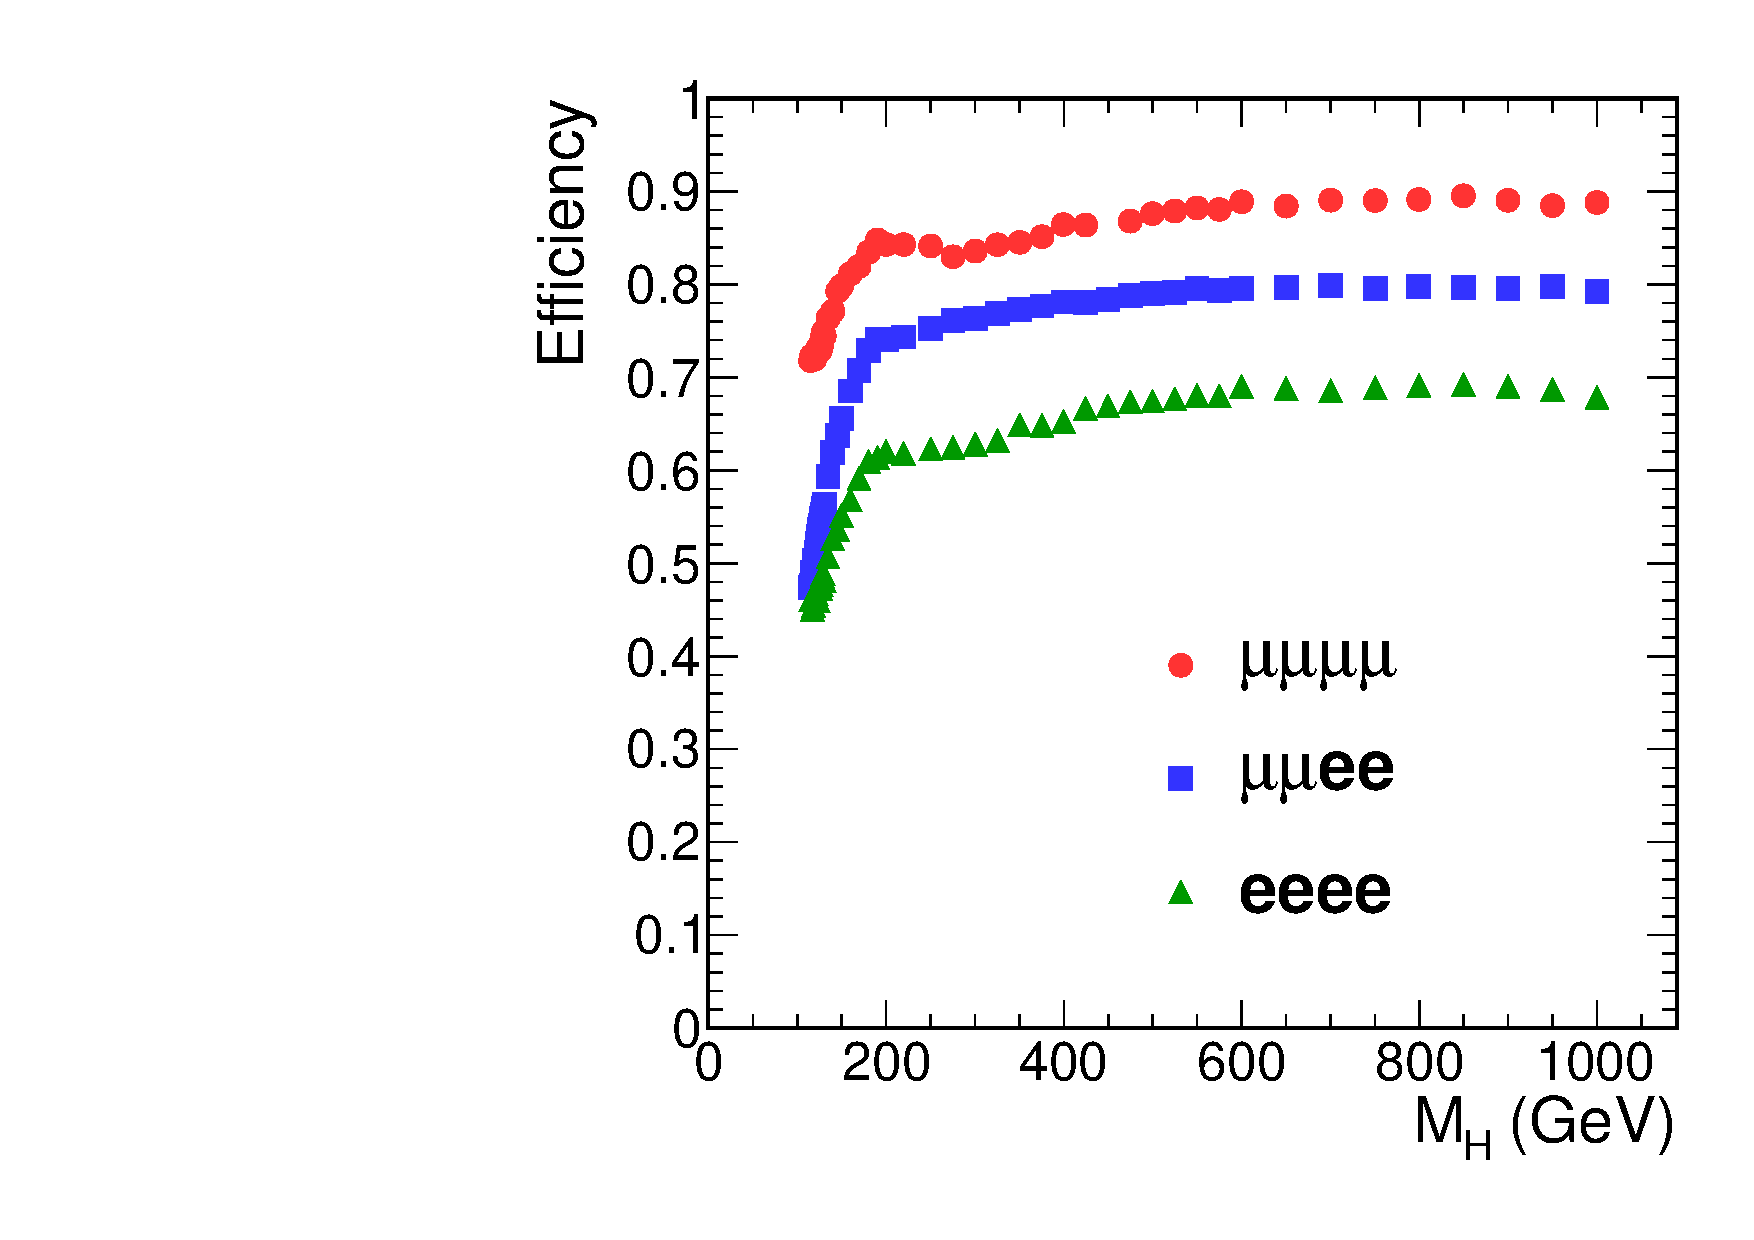
\includegraphics[width=0.80\textwidth]{higgs_eff}
\caption[Final selection efficiency, as a function of Higgs mass.]{Final selection efficiency for each final
state, as a function of the Higgs mass. Efficiency is defined as the number of
selected events to the number of events produced within the geometrical and
kinematic requirements of the analysis.}
\label{fig:selEff}
\end{figure}



%\section{Acceptance}
\section{Signal and background modelling}

In the search for a Standard Model Higgs boson, the differential distribution
(with respect to the four-lepton invariant mass) is factorized as:
\begin{equation}
    \label{eqn:higgsShape}
    \frac{dN}{dM_{\ell\ell\ell\ell}} = C_{\epsilon} \cdot N^{MC}(m_H)
    \cdot F_H(M_{\ell\ell\ell\ell} | m_H)
\end{equation}
where $C_\epsilon$ is the product of the leptonic correction factors (described
in section~\ref{sub:scale_factors}), $m_H$ is the hypothesized Higgs boson mass,
and $F_H$ is the probability density function of the Higgs mass distribution.
This function is a convolution of a relativistic Breit-Wigner
function~\footnote{$\frac{\Gamma_{gg}(m_{4\ell})\cdot\Gamma_ZZ(m_{4\ell})\cdot m_{4\ell}}
{(m_{4\ell}^2-m_{H}^2)^2+m_{4\ell}^2\cdot\Gamma^2(m_{4\ell})}$} with a
double Crystal Ball function~\footnote{$\begin{cases} 
A \cdot (B+|\xi|)^{-n_L} &\text{for } \xi < \alpha_L \\ 
A \cdot (B+|\xi|)^{-n_R} &\text{for } \xi > \alpha_R \\ 
exp(-\xi^2/2), & \text{for } \alpha_L \le \xi \le \alpha_R  \\
\xi = (m_{4\ell} - m_{H} - \Delta m_{H} )/ \sigma_m
\end{cases}$}, added to account for the low- and high-side tails
from bremsstrahlung effects and detector mismeasurement effects.
The shape parameters are fit using the available Monte Carlo simulation samples,
then a secondary fit to the shape parameters is used in extracting shape values
between the generated samples. This allows a smoothly varying shape to be used
as input across an arbitrary Higgs mass hypothesis range.
A full description of the shape and its parameters is given
in~\cite{higgsSigShape}.

For a low ($< 400~GeV$) mass Higgs hypothesis, the implicit zero-width
assumption used in the fitting procedure above holds valid. However, as the
Higgs width becomes wider, this assumption breaks down. As a result, all cross
sections and lineshapes in the high-mass Higgs hypotheses utilize the
\emph{Complex Pole Scheme (CPS)}~\cite{higgsLineshape}. Additionally,
interference between Higgs and $gg\rightarrow ZZ$ production causes a significant
deformation in the invariant mass distribution. This is corrected (and
uncertainties computed) using the scheme proposed in
~\cite{higgsHighMassInterference}. The uncertainties are explained in
Section~\ref{sec:systematics}.

In the Higgs search, the ZZ background is treated in a way similar to the Higgs
signal (Eqn.\ref{eqn:higgsShape}). However the shape, $F_H$, is replaced by:

\begin{equation*}
    \frac{dN_{qq\rightarrow ZZ}}{dM_{\ell\ell\ell\ell}} = C_{\epsilon} \cdot N^{MC}(m_H)
        \cdot ( f_1 + f_2 + f_3 )
\end{equation*}
\begin{equation*}
    \frac{dN_{gg\rightarrow ZZ}}{dM_{\ell\ell\ell\ell}} = C_{\epsilon} \cdot N^{MC}(m_H)
        \cdot ( f_1 + f_2 )
\end{equation*}
\begin{equation*}
    f_1(m, \vec{a}) = \left(0.5 + 0.5
        erf(\frac{m-a_1}{a_2}) \right ) \cdot \frac{a_4}{1+\exp{(m-a_1)/a_3}}
\end{equation*}
\begin{equation*}
    f_2(m, \vec{b}) = \left(0.5 + 0.5
        erf(\frac{m-b_1}{b_2}) \right ) \cdot \left (
        \frac{b_4}{1+\exp{(m-b_1)/b_3}} + \frac{b_6}{1+\exp{(m-b_1)/b_5}}
        \right)
\end{equation*}
\begin{equation}
    f_3(m, \vec{c}) = \left(0.5 + 0.5
        erf(\frac{m-c_1}{c_2}) \right ) \cdot \frac{c_4}{1+\exp{(m-c_1)/c_3}}
\end{equation}

\section{Systematic Uncertainties}
\label{sec:systematics}

\subsection{Higgs Signal Simulation}
Systematic uncertainties for the Higgs samples effect either the overall
yield or the shape of the signal. Uncertainties that enter only through the
yield include:
\begin{itemize}
\item Uncertainty on Higgs production cross section, $H\rightarrow ZZ$, and
    $ZZ\rightarrow 4\ell$ branching ratios.
\item Uncertainty on acceptance measurements
\item Uncertainties on data-to-MC correction factors
\end{itemize}
while uncertainties that impact the signal shape are:
\begin{itemize}
    \item The theoretical uncertainties in the pdf of the Higgs shape, $F_H(M_{\ell\ell\ell\ell} | m_H)$
    \item Uncertainties in the modelling of detector effects within the double
        Crystal ball fit
\end{itemize}

The uncertainty on the Higgs production cross section arises from the PDF and
$\alpha_s$ (the strong force coupling strength) errors in addition to
uncertainties in the QCD renormalization ($\mu_R$)  and 
factorization ($\mu_F$) scales (which are theoretical constructs to remove
divergent cross section calculations).
These values, in addition to the cross sections themselves, are provided by the
LHC working group~\cite{lhcHiggsHandbook}.  Effects due to the acceptance are
measured using MCFM, adjusting $\mu_R$ and $\mu_F$ up and down by a factor of
two and calculating the total change in acceptance. These uncertainties are
found to be at the 0.1-0.2\% level, and are neglected. PDF and $\alpha_s$
effects on the acceptance are measured using the PDF4LHC
prescription~\cite{PDF4LHC}, in which three different PDF sets are used
(\cite{ct10}, \cite{MSTW08}, \cite{nnPDF}), with the maximum differences being
the final systematic effect. This is found to be a fairly flat effect across all
Higgs masses, and a flat 2\% systematic is applied.

Shape systematic uncertainties are measured by utilizing alternate shape
hypotheses, refitting the samples, and taking the envelope of the outcomes as
the systematic error.

The data-to-MC scale factors corrections, obtained from the tag and probe method
outlined in Section~\ref{sub:scale_factors}, are applied on a per-lepton basis.
Each lepton provides an additional weight factor that is applied when extracting
the Monte Carlo yield. Uncertainties in the correction factor measurements
(coming from shape and modelling uncertainties in the tag and probe process) are
propagated into a final uncertainty by running, for each MC sample, a batch of
500 toy MC experiments. For each, the correction factor is extracted via a
Gaussian, centered at the data/MC ratio and with a $\sigma$ equal to the
associated error. The final systematic uncertainty on the MC yields is defined
to be the RMS of the distribution of these pseudoexperiments.


\subsection{ZZ Simulation}
Many of the systematic uncertainties on ZZ are similar to those for the Higgs signal.
Uncertainties on the total yields are due primarily to the theoretical
uncertainties, PDF+$\alpha_s$ and QCD scales, and the instrumental uncertainties
on the data-MC scaling.

PDF+$\alpha_s$ uncertainties are again evaluated using the PDF4LHC method, as
with the Higgs sample. The $qq \rightarrow ZZ$ and $gg\rightarrow ZZ$
errors are evaluated separately, and vary roughly with the square root of the
$M_{\ell\ell\ell\ell}$:
\begin{equation*}
    qq\rightarrow ZZ : \kappa (M_{\ell\ell\ell\ell}) = 1 + 0.0035
    \sqrt{M_{\ell\ell\ell\ell} - 30}
\end{equation*}
\begin{equation}
    gg\rightarrow ZZ : \kappa (M_{\ell\ell\ell\ell}) = 1 + 0.0066
    \sqrt{M_{\ell\ell\ell\ell} - 10}
\end{equation}

QCD scale uncertainties are treated the same way, measuring the envelope of errors
resulting from scaling $\mu_F$ and $\mu_R$, with uncertainties
parameterized as:
\begin{equation*}
    qq\rightarrow ZZ : \kappa (M_{\ell\ell\ell\ell}) = 1.00 + 0.01\sqrt{(M_{\ell
    \ell\ell\ell} -20)/13}
\end{equation*}
\begin{equation*}
    gg\rightarrow ZZ : \kappa (M_{\ell\ell\ell\ell}) = 1.04 + 0.10\sqrt{(M_{\ell
    \ell\ell\ell} +40)/40}
\end{equation*}

\subsection{Systematic Uncertainties on Reducible Backgrounds}
The uncertainties on the reducible background estimates come primarily from the
limited statistics in the regions where fake rates are applied, the
uncertainties in the measured fake rates, and the uncertainty in the
difference in background sources while migrating between the regions. MC closure
tests and OS/SS checks were conducted, but were limited by statistics. Alternate
reducible BG calculations were conducted, and a conservative estimate of 30-50\%
was applied (depending on the final state).

\subsection{Global Uncertainties in MC-driven estimates}
In addition to the uncertainties outlined above, there are two global effects
which impact the yield extraction from the Monte Carlo simulated samples. First,
uncertainties in the measurement in the integrated luminosity were found to be
4.4\%~\cite{lumi}. Additionally, the uncertainty on the trigger corrections (which come from
tag and probe measurements) is evaluated to 1.5\%~\cite{zzHiggsMoriond}.

\section{Summary}
The selection criteria for the search of a $ZZ\rightarrow \ell\ell\ell\ell$
final state is designed to be as loose as possible in order to maximize the
efficiency of this clean, though low-probability, final state. The final
selection criteria on electrons, muons, and Z boson candidates are summarized in
Table~\ref{tab:selection_criteria}.

\begin{table}[h]
\centering
\begin{tabular}{|c|c|}
\hline
\multicolumn{2}{|c|}{Electron selection} \\
\hline
Kinematics & $p_T > 7~GeV$, $|\eta| < 2.5$ \\
Identification & MVA ID as defined above. \\ 
Isolation & $rho$-corrected relative isolation < 0.40 \\
\hline
\multicolumn{2}{|c|}{Muon selection} \\
\hline
Kinematics & $p_T > 5~GeV$, $|\eta| < 2.4$ \\
Identification & (Global OR Tracker), PF Muon \\
Isolation & $rho$-corrected relative isolation < 0.40 \\
\hline
\multicolumn{2}{|c|}{Z Candidate Selections} \\
\hline
Higgs search (low-mass) & $40 < M_{Z1} < 120~GeV$ \\
                        & $12 < M_{Z2} < 120~GeV$ \\
SM ZZ and aTGC analysis (high-mass) & $60 < M_{Z1} < 120~GeV$ \\
                        & $60 < M_{Z2} < 120~GeV$ \\
\hline
\end{tabular}
\caption[Summary of the selection criteria.]{Summary of the selection criteria.}
\label{tab:selection_criteria}
\end{table}

Additionally, careful consideration of systematic uncertainties, both on
expected yields and shapes of signals and background, have been evaluated. These
uncertainties are summarized in Table~\ref{tab:systematics}.

\begin{table}[h]
\small
\centering
\begin{tabular}{|c|c|c|c|c|c||c|c|}
    \hline
    & ggH & VBF & WH & ZH & ttH & $qqZZ$ & $ggZZ$ \\
    \hline
    $gg$ pdf uncertainty & 7.2-9.2 & - & - & - & 0-9.8 & - & 10 \\
    $qq / q\overline q$ pdf uncertainty & - & 1.2-1.8 & 0-4.5 & 0-5.0 & - & 5 &
    - \\
    QCD Scale & 5.5-7.9 & 0.1-0.2 & 0-0.6 & 9-1.5 & 0-8.8 & 2.6-6.7 & 24-44 \\
    $H\rightarrow 4l$ BR & 2 & 2 & 2 & 2 & 2 & - & - \\
    \hline
    CB mean parameterization  & \multicolumn{5}{c||}{0.4} & - & - \\
    CB $\sigma$ parameterization & \multicolumn{5}{c||}{ 20 } & - & - \\
    CB $\alpha$ parameterization & \multicolumn{5}{c||}{ 20 } & - & - \\
    \hline
    Luminosity & \multicolumn{7}{c|}{ 4.2 } \\ 
    Trigger & \multicolumn{7}{c|}{ 1.5 } \\
    Electron efficiency scale & \multicolumn{7}{c|}{ 6.2-11} \\
    Muon efficiency scale & \multicolumn{7}{c|} { 1.9 } \\
\hline
\end{tabular}
\caption[Summary of the systematic uncertainties.]{Summary of the systematic
uncertainties.}
\label{tab:systematics}
\end{table}

